\documentclass[a4paper,12pt]{article}
   % Packages and definitions:
   % {
      \usepackage{float}
      \usepackage[english]{babel}
      \usepackage[utf8]{inputenc}
      \usepackage{amsmath}
      \usepackage{mathtools}
      \usepackage{amssymb}
      \usepackage{color}
      \usepackage{subcaption}
      \usepackage{booktabs}
      \usepackage{tikz}
      \usepackage{multirow}
      \usepackage{siunitx}
      \usetikzlibrary{decorations.pathreplacing}
      \usepackage{graphicx,epstopdf}
      \usepackage{cleveref}
      \usepackage{collcell} % loads array
      \usepackage{listings}
      \usepackage{algorithm}
      \usepackage{algpseudocode}
      \newcolumntype{m}{>{$} r <{$}}
      \newcolumntype{u}{>{$[\collectcell\si} l <{\endcollectcell]$}}
      \newcommand{\approxtext}[1]{\ensuremath{\stackrel{\text{#1}}{=}}}
      \newcommand{\matr}[1]{\mathbf{#1}}
      \newcommand{\partt}[2]{\ensuremath{\dfrac{\partial {#1}}{\partial {#2}}}}
      \renewcommand{\d}[1]{\ensuremath{\operatorname{d}\!{#1}}} % non-italized differentials
      \newcommand{\h}[0]{\ensuremath{\hbar}} % hbar
      \newcommand{\qed}[0]{\ensuremath{\tag*{$\square$}}} % QED square
      \def\changemargin#1#2{\list{}{\rightmargin#2\leftmargin#1}\item[]}
      \let\endchangemargin=\endlist 
      \usepackage{amsthm}
      \theoremstyle{plain}
      \newtheorem{thm}{theorem} % reset theorem numbering for each chapter
      \theoremstyle{definition}
      \newtheorem{defn}[thm]{definition} % definition numbers are dependent on theorem numbers
      \newtheorem{exmp}[thm]{example} % same for example numbers
      \bibliographystyle{natbib}
      \renewcommand{\theequation}{\thesection.\arabic{equation}}
      \newcommand{\ts}{\textsuperscript} 

      \definecolor{dkgreen}{rgb}{0,0.6,0}
      \definecolor{gray}{rgb}{0.5,0.5,0.5}
      \definecolor{mauve}{rgb}{0.58,0,0.82}

      \lstset{frame=tb,
        language=Java,
        aboveskip=3mm,
        belowskip=3mm,
        showstringspaces=false,
        columns=flexible,
        basicstyle={\small\ttfamily},
        numbers=none,
        numberstyle=\tiny\color{gray},
        keywordstyle=\color{blue},
        commentstyle=\color{dkgreen},
        stringstyle=\color{mauve},
        breaklines=true,
        breakatwhitespace=true,
        tabsize=3
      }
% }
\title
{
	\textbf
	{
      Laboratory exercise 2: \\Chemical reactions
   }
}

\author{Henrik Åhl}
\date{\today}

\begin{document}
\begin{titlepage}
	
   \maketitle 
	\begin{center}
		\phantom{a}
		{Department of Astronomy and Theoretical Physics, Lund University}
		\\[2cm]
		{Project supervised by Behruz Bozorg}
		\vfill
		\includegraphics[height=4cm]{logocLUeng.pdf}
	\end{center}
	\thispagestyle{empty} % do not count pages just yet

\end{titlepage}

\section{Introduction}
   In this report we model and analyze different chemical reactions and
   investigate how different setups and different models might affect the
   outcome of our simulations -- i.e. the occurence of equilibrium states,
   oscillating behaviour and general dynamics within the systems in question.

   Since chemical reactions are complex, we here present iterative enhancements 
   of simple models in order to succesively better approximate the intended 
   behaviour of our chemical reactions in question. 

\section{Theory and methodology}
	\setcounter{equation}{0}
   \subsection{A model using two state reactions}
      In a so called \emph{two state reaction}, reactions can happen, as the name
      suggests, between two different states, and is most easily represented by the
      chemical equation 
         \begin{align}
            A \xrightleftharpoons[k_-]{k_+} B
         \end{align}
      between the two states $A$ and $B$. Resultingly, the concentration change in
      say $A$ can then be described naively by
      \begin{align}
         \frac{\partial [A]}{\partial t} = k_- [B] - k_+ [A]
         \label{eq:change_A}
      \end{align}
      whereas the change in $[B]$ is simply the negative of this. 

      How this reaction actually takes place is determined by an energy barrier
      $\Delta G^{\ddagger}$, where $\Delta G = \sum_i \mu_i \d N_i$ is the change
      in Gibbs' free energy under constant temperature and pressure, that must be overcome 
      for the reacting molecule, or \emph{reactant}, to go into the inbetween state 
      of transition. Our above introduced rate constants $k_+$ and $k_-$ are thusly 
      given by 
      \begin{align}
         k_+ = \frac{k_B}{h} e^{-\beta\Delta G^{\ddagger}}
         \label{eq:k_def}
      \end{align}
      for the forward rate, and correspondingly for $k_-$. Here $k_B$ is the
      Boltzmann constant, while $h$ is the unreduced Planck constant.

      At equilibrium, the change in concentration between the two states is equal,
      so that 

         \begin{align}
            \frac{[B]}{[A]} = \frac{k_+}{k_-} \equiv K_{eq}. 
            \label{eq:K_eq_def}
         \end{align}
      This result demonstrates a feature of how the activation barrier affects
      the level of equilibrium -- it simply does not, as the quota between the
      rates will remain constant. It does however seem reasonable that it would affect
      the time needed for an equilibrium state to be established, although the
      model does not provide any telling information about this. 

   \subsection{Catalyzed reaction}
      Enzymes can act as catalysts for reactions by binding to the different
      molecules, lowering their effective potential barrier. 
      
      A simplified model for this sort of reaction, between our earlier states 
      $A$ and $B$ can be described by the reaction formula
         \begin{align}
            A + E~\stackrel{k_+}{\rightharpoonup}~B + E
            \label{eq:enzymes}
         \end{align}
      so that the enzyme itself is unchanged after the transition. 
     
      In this case, the change in the concentration of the different substrates
      can collectively be described analogously to the two-state case by
         \begin{align*}
            \partt{[A]}{t} &= -k_+[A][E] \\
            \partt{[B]}{t} &= - \partt{[A]}{t} \\
            \partt{[E]}{t} &= 0
         \end{align*}
      where the product of the concentrations is due to the effective reactions
      being able to take place. Notably, as $[A]$ would tend towards infinity,
      so would the the rate of change. 
      
      In a more evolved model on the other
      hand, the reaction could instead be written as
         \begin{align}
            A + E \xrightleftharpoons[k_2]{k_1} AE \stackrel{k_+}{\rightharpoonup}
            = B + E 
            \label{eq:transition_state}
         \end{align}
      to account for the inbetween state where the enzyme E binds to A, forming
      a substrate complex. This reaction would in turn be more aptly described
      by the equations
         \begin{align*}
            \partt{[A]}{t} &= -k_1[A][E] + k_2[AE] \\
            \partt{[E]}{t} &= -k_1[A][E] + k_2[AE] + k_+[AE] \\
            \partt{[AE]}{t} &= -k_2[AE] + k_1[A][E] - k_+[AE] \\
            \partt{[B]}{t} &= k_+[AE]
         \end{align*}
      in exactly the same manner as before. Reasonably, this would limit the
      rate at which $[A]$ changes, though it however still contains anomalies
      with respect to exactly this extreme.

      In the so called Michaelis-Menten equation however, also the enzymes'
      working speed comes into play, as it before has ben implicitly assumed to
      be infinite. In this case, the concentration of the substrate complex is
      assumed to be constant, as well as the enzyme itself, so that the
      following conditions hold:
         \begin{align*}
            \partt{[AE]}{t} &= -k_1[A][E] + k_2[AE] + k_+[AE] = 0 \\
            [E^{tot}] &= [E] + [AE] 
         \end{align*}
         Here $E^{tot}$ is, as the name suggests, the total amount of enzyme
         available in any form. Applying this to our
         earlier set of equations we attain
         \begin{align*}
            (k_2 + k_+)[AE] &= k_1[A]([E^{tot}] - [AE]) 
         \end{align*}
      and thus ultimately
         \begin{align*}
            \partt{[B]}{t} &= k_+ \frac{[A][E^{tot}]}{k_2 + k_1[A] + k_+}.
         \end{align*}
      Defining 
         \begin{align*}
            v_{max} \equiv k_+ [E^{tot}] \\
            k_m \equiv \frac{k_2 + k_+}{k_1}
         \end{align*}
      we achieve the final expression
         \begin{align*}
            v = v_{max} \frac{[A]}{k_m + [A]}.
         \end{align*}

      \subsection{Diffusion}
         Substrates mainly travel through diffusion between cells, so it is
         therefore necessary to be able to model also this phenomenon. In a
         one-dimensional case, this is a very simple procedure. Just assume that
         the cells are lain out in a vector-like structure, so that a typical
         cell with concentration $c_i$ have the two neighbors with the dito $c_{i-1}$ 
         and $c_{i+1}$. The diffusion, i.e. the rate of transport between the
         cells, is then easiliy described by the equation 
            \begin{align}
               \frac{\d c_i}{\d t} = D(c_{i-1} - 2c_i + c_{i+1})
               \label{eq:diff}
            \end{align}
         which can be proven quite trivially through assuming that all particles
         move randomly every time step with a probability $p$, and do not have significant bias towards either
         direction. Let the number of particles in a cell $i$ be defined by the value $N_i$. 
         The number of particles moving into this cell $i$ from both neighbors must then 
         equal $pN_{i-1} + p N_{i+1}$, wheras the flow out of the cell must be
         $2pN_i$. This gives the resulting equation 
            \begin{align*}
               \frac{\d N_i}{\d t} = p(N_{i-1} - 2N_i + N_{i+1})
            \end{align*}
         where if we divide by the volume (assuming it common across the
         different cells), the concentration is gained. This looks very much
         like the discretized case of the diffusion equation apart from the
         fact that we here cannot relate our constant $D$ to physical
         entities, such as distance and time.



      \subsection{The brusselator}
         Introducing the brusselator, chemical reactions can be modelled
         according to the reaction equations

         \begin{align*}
            A        &\stackrel{k_1}{\rightharpoonup} X \\
            2X + Y   &\stackrel{k_2}{\rightharpoonup} 3X \\
            B + X    &\stackrel{k_3}{\rightharpoonup} Y + C \\
            X        &\stackrel{k_4}{\rightharpoonup} D
         \end{align*}
         where $A$, and $B$ are held constant. For the substrates of interest,
         $X$ and $Y$, the time derivatives are given as
         \begin{align*}
            \partt{[X]}{t} &= k_1[A] + k_2[X]^2[Y] - k_3[B][X] - k_4[X] \\
            \partt{[Y]}{t} &= -k_2[X]^2[Y] + k_3[B][X]
         \end{align*}
         where we can note for mere curiosity that the absence of either of $A$ 
         and $B$ would imply that the concentration of both $X$ and $Y$ would go 
         towards 0. Whereas the lack of the ``outflow'' $k_4$ would mean that
         both the concentration of $X$ and $Y$ would tend towards infinity
         instead.~\cite{lecnotes}

\section{Results and conclusions}

      Calculating the forward rate constant using numerical values of 
      $\mu_A^0 = 8, \mu_B^0 = 3$ and $\Delta G^{\ddagger} = 75$, with all units
      measured in kJ/mol, as well as approximate room temperature, renders the forward
      rate as $k_+ = 0.89$, whereas the backward rate correspondingly assumes
      the a value of $k_- = 6.01 \cdot 10^{-3}$. 

      Simulation results are visible in \cref{fig:twostate} and
      \cref{fig:twostate_2}, where the dynamics of our system is apparent. Here
      the flux in the forward direction is many times larger than the backward
      flux, why the equlibrium state, i.e. the state where the concentrations
      converge, biases $[B]$ so heavily. When the initial concentrations are
      altered, the translation is clearly visible, as is expected of our simple
      model. 

      \begin{figure}[H]
         \vspace*{1cm}
         \hspace*{-2cm}
         \centering
         \begin{minipage}[t]{.6\textwidth}		
            \vspace{0pt}
            \centering
            \resizebox{\columnwidth}{!}{% GNUPLOT: LaTeX picture with Postscript
\begingroup
  \makeatletter
  \providecommand\color[2][]{%
    \GenericError{(gnuplot) \space\space\space\@spaces}{%
      Package color not loaded in conjunction with
      terminal option `colourtext'%
    }{See the gnuplot documentation for explanation.%
    }{Either use 'blacktext' in gnuplot or load the package
      color.sty in LaTeX.}%
    \renewcommand\color[2][]{}%
  }%
  \providecommand\includegraphics[2][]{%
    \GenericError{(gnuplot) \space\space\space\@spaces}{%
      Package graphicx or graphics not loaded%
    }{See the gnuplot documentation for explanation.%
    }{The gnuplot epslatex terminal needs graphicx.sty or graphics.sty.}%
    \renewcommand\includegraphics[2][]{}%
  }%
  \providecommand\rotatebox[2]{#2}%
  \@ifundefined{ifGPcolor}{%
    \newif\ifGPcolor
    \GPcolorfalse
  }{}%
  \@ifundefined{ifGPblacktext}{%
    \newif\ifGPblacktext
    \GPblacktexttrue
  }{}%
  % define a \g@addto@macro without @ in the name:
  \let\gplgaddtomacro\g@addto@macro
  % define empty templates for all commands taking text:
  \gdef\gplbacktext{}%
  \gdef\gplfronttext{}%
  \makeatother
  \ifGPblacktext
    % no textcolor at all
    \def\colorrgb#1{}%
    \def\colorgray#1{}%
  \else
    % gray or color?
    \ifGPcolor
      \def\colorrgb#1{\color[rgb]{#1}}%
      \def\colorgray#1{\color[gray]{#1}}%
      \expandafter\def\csname LTw\endcsname{\color{white}}%
      \expandafter\def\csname LTb\endcsname{\color{black}}%
      \expandafter\def\csname LTa\endcsname{\color{black}}%
      \expandafter\def\csname LT0\endcsname{\color[rgb]{1,0,0}}%
      \expandafter\def\csname LT1\endcsname{\color[rgb]{0,1,0}}%
      \expandafter\def\csname LT2\endcsname{\color[rgb]{0,0,1}}%
      \expandafter\def\csname LT3\endcsname{\color[rgb]{1,0,1}}%
      \expandafter\def\csname LT4\endcsname{\color[rgb]{0,1,1}}%
      \expandafter\def\csname LT5\endcsname{\color[rgb]{1,1,0}}%
      \expandafter\def\csname LT6\endcsname{\color[rgb]{0,0,0}}%
      \expandafter\def\csname LT7\endcsname{\color[rgb]{1,0.3,0}}%
      \expandafter\def\csname LT8\endcsname{\color[rgb]{0.5,0.5,0.5}}%
    \else
      % gray
      \def\colorrgb#1{\color{black}}%
      \def\colorgray#1{\color[gray]{#1}}%
      \expandafter\def\csname LTw\endcsname{\color{white}}%
      \expandafter\def\csname LTb\endcsname{\color{black}}%
      \expandafter\def\csname LTa\endcsname{\color{black}}%
      \expandafter\def\csname LT0\endcsname{\color{black}}%
      \expandafter\def\csname LT1\endcsname{\color{black}}%
      \expandafter\def\csname LT2\endcsname{\color{black}}%
      \expandafter\def\csname LT3\endcsname{\color{black}}%
      \expandafter\def\csname LT4\endcsname{\color{black}}%
      \expandafter\def\csname LT5\endcsname{\color{black}}%
      \expandafter\def\csname LT6\endcsname{\color{black}}%
      \expandafter\def\csname LT7\endcsname{\color{black}}%
      \expandafter\def\csname LT8\endcsname{\color{black}}%
    \fi
  \fi
  \setlength{\unitlength}{0.0500bp}%
  \begin{picture}(7200.00,5040.00)%
    \gplgaddtomacro\gplbacktext{%
      \colorrgb{0.42,0.42,0.42}%
      \put(946,704){\makebox(0,0)[r]{\strut{}0.00}}%
      \colorrgb{0.42,0.42,0.42}%
      \put(946,1518){\makebox(0,0)[r]{\strut{}0.04}}%
      \colorrgb{0.42,0.42,0.42}%
      \put(946,2332){\makebox(0,0)[r]{\strut{}0.08}}%
      \colorrgb{0.42,0.42,0.42}%
      \put(946,3147){\makebox(0,0)[r]{\strut{}0.12}}%
      \colorrgb{0.42,0.42,0.42}%
      \put(946,3961){\makebox(0,0)[r]{\strut{}0.16}}%
      \colorrgb{0.42,0.42,0.42}%
      \put(946,4775){\makebox(0,0)[r]{\strut{}0.20}}%
      \colorrgb{0.42,0.42,0.42}%
      \put(1078,484){\makebox(0,0){\strut{} 0}}%
      \colorrgb{0.42,0.42,0.42}%
      \put(2223,484){\makebox(0,0){\strut{} 2}}%
      \colorrgb{0.42,0.42,0.42}%
      \put(3368,484){\makebox(0,0){\strut{} 4}}%
      \colorrgb{0.42,0.42,0.42}%
      \put(4513,484){\makebox(0,0){\strut{} 6}}%
      \colorrgb{0.42,0.42,0.42}%
      \put(5658,484){\makebox(0,0){\strut{} 8}}%
      \colorrgb{0.42,0.42,0.42}%
      \put(6803,484){\makebox(0,0){\strut{} 10}}%
      \colorrgb{0.42,0.42,0.42}%
      \put(176,2739){\rotatebox{-270}{\makebox(0,0){\strut{}Concentration}}}%
      \colorrgb{0.42,0.42,0.42}%
      \put(3940,154){\makebox(0,0){\strut{}Time}}%
      \colorrgb{0.42,0.42,0.42}%
      \put(3940,4665){\makebox(0,0){\strut{}}}%
    }%
    \gplgaddtomacro\gplfronttext{%
      \csname LTb\endcsname%
      \put(5804,4602){\makebox(0,0)[r]{\strut{}A}}%
      \csname LTb\endcsname%
      \put(5804,4382){\makebox(0,0)[r]{\strut{}B}}%
    }%
    \gplbacktext
    \put(0,0){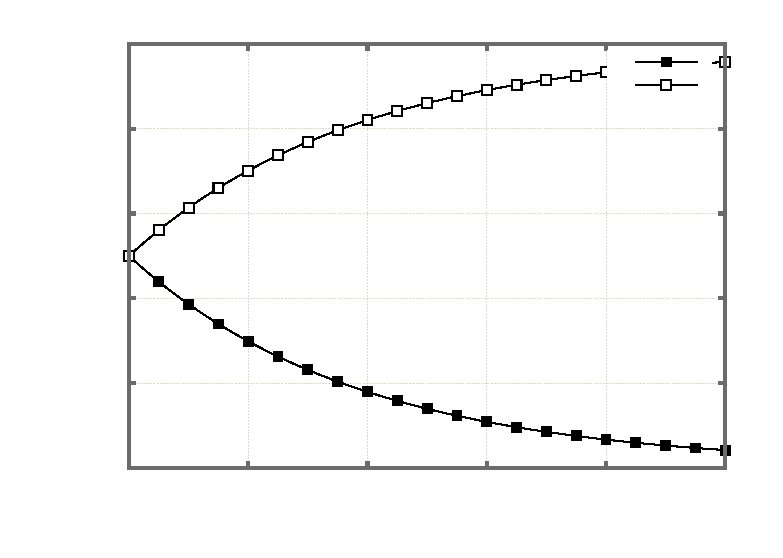
\includegraphics{twostate}}%
    \gplfronttext
  \end{picture}%
\endgroup
}
            \caption{Simulation of a two-state system with equal initial
            concentration.}
            \label{fig:twostate}
         \end{minipage}~\hspace*{1em}
         \begin{minipage}[t]{.6\textwidth}		
            \vspace{0pt}
            \centering
            \resizebox{\columnwidth}{!}{% GNUPLOT: LaTeX picture with Postscript
\begingroup
  \makeatletter
  \providecommand\color[2][]{%
    \GenericError{(gnuplot) \space\space\space\@spaces}{%
      Package color not loaded in conjunction with
      terminal option `colourtext'%
    }{See the gnuplot documentation for explanation.%
    }{Either use 'blacktext' in gnuplot or load the package
      color.sty in LaTeX.}%
    \renewcommand\color[2][]{}%
  }%
  \providecommand\includegraphics[2][]{%
    \GenericError{(gnuplot) \space\space\space\@spaces}{%
      Package graphicx or graphics not loaded%
    }{See the gnuplot documentation for explanation.%
    }{The gnuplot epslatex terminal needs graphicx.sty or graphics.sty.}%
    \renewcommand\includegraphics[2][]{}%
  }%
  \providecommand\rotatebox[2]{#2}%
  \@ifundefined{ifGPcolor}{%
    \newif\ifGPcolor
    \GPcolorfalse
  }{}%
  \@ifundefined{ifGPblacktext}{%
    \newif\ifGPblacktext
    \GPblacktexttrue
  }{}%
  % define a \g@addto@macro without @ in the name:
  \let\gplgaddtomacro\g@addto@macro
  % define empty templates for all commands taking text:
  \gdef\gplbacktext{}%
  \gdef\gplfronttext{}%
  \makeatother
  \ifGPblacktext
    % no textcolor at all
    \def\colorrgb#1{}%
    \def\colorgray#1{}%
  \else
    % gray or color?
    \ifGPcolor
      \def\colorrgb#1{\color[rgb]{#1}}%
      \def\colorgray#1{\color[gray]{#1}}%
      \expandafter\def\csname LTw\endcsname{\color{white}}%
      \expandafter\def\csname LTb\endcsname{\color{black}}%
      \expandafter\def\csname LTa\endcsname{\color{black}}%
      \expandafter\def\csname LT0\endcsname{\color[rgb]{1,0,0}}%
      \expandafter\def\csname LT1\endcsname{\color[rgb]{0,1,0}}%
      \expandafter\def\csname LT2\endcsname{\color[rgb]{0,0,1}}%
      \expandafter\def\csname LT3\endcsname{\color[rgb]{1,0,1}}%
      \expandafter\def\csname LT4\endcsname{\color[rgb]{0,1,1}}%
      \expandafter\def\csname LT5\endcsname{\color[rgb]{1,1,0}}%
      \expandafter\def\csname LT6\endcsname{\color[rgb]{0,0,0}}%
      \expandafter\def\csname LT7\endcsname{\color[rgb]{1,0.3,0}}%
      \expandafter\def\csname LT8\endcsname{\color[rgb]{0.5,0.5,0.5}}%
    \else
      % gray
      \def\colorrgb#1{\color{black}}%
      \def\colorgray#1{\color[gray]{#1}}%
      \expandafter\def\csname LTw\endcsname{\color{white}}%
      \expandafter\def\csname LTb\endcsname{\color{black}}%
      \expandafter\def\csname LTa\endcsname{\color{black}}%
      \expandafter\def\csname LT0\endcsname{\color{black}}%
      \expandafter\def\csname LT1\endcsname{\color{black}}%
      \expandafter\def\csname LT2\endcsname{\color{black}}%
      \expandafter\def\csname LT3\endcsname{\color{black}}%
      \expandafter\def\csname LT4\endcsname{\color{black}}%
      \expandafter\def\csname LT5\endcsname{\color{black}}%
      \expandafter\def\csname LT6\endcsname{\color{black}}%
      \expandafter\def\csname LT7\endcsname{\color{black}}%
      \expandafter\def\csname LT8\endcsname{\color{black}}%
    \fi
  \fi
  \setlength{\unitlength}{0.0500bp}%
  \begin{picture}(7200.00,5040.00)%
    \gplgaddtomacro\gplbacktext{%
      \colorrgb{0.42,0.42,0.42}%
      \put(946,704){\makebox(0,0)[r]{\strut{}0.00}}%
      \colorrgb{0.42,0.42,0.42}%
      \put(946,1383){\makebox(0,0)[r]{\strut{}0.08}}%
      \colorrgb{0.42,0.42,0.42}%
      \put(946,2061){\makebox(0,0)[r]{\strut{}0.16}}%
      \colorrgb{0.42,0.42,0.42}%
      \put(946,2740){\makebox(0,0)[r]{\strut{}0.24}}%
      \colorrgb{0.42,0.42,0.42}%
      \put(946,3418){\makebox(0,0)[r]{\strut{}0.32}}%
      \colorrgb{0.42,0.42,0.42}%
      \put(946,4097){\makebox(0,0)[r]{\strut{}0.40}}%
      \colorrgb{0.42,0.42,0.42}%
      \put(946,4775){\makebox(0,0)[r]{\strut{}0.48}}%
      \colorrgb{0.42,0.42,0.42}%
      \put(1078,484){\makebox(0,0){\strut{} 0}}%
      \colorrgb{0.42,0.42,0.42}%
      \put(2223,484){\makebox(0,0){\strut{} 2}}%
      \colorrgb{0.42,0.42,0.42}%
      \put(3368,484){\makebox(0,0){\strut{} 4}}%
      \colorrgb{0.42,0.42,0.42}%
      \put(4513,484){\makebox(0,0){\strut{} 6}}%
      \colorrgb{0.42,0.42,0.42}%
      \put(5658,484){\makebox(0,0){\strut{} 8}}%
      \colorrgb{0.42,0.42,0.42}%
      \put(6803,484){\makebox(0,0){\strut{} 10}}%
      \colorrgb{0.42,0.42,0.42}%
      \put(176,2739){\rotatebox{-270}{\makebox(0,0){\strut{}Concentration}}}%
      \colorrgb{0.42,0.42,0.42}%
      \put(3940,154){\makebox(0,0){\strut{}Time}}%
      \colorrgb{0.42,0.42,0.42}%
      \put(3940,4665){\makebox(0,0){\strut{}}}%
    }%
    \gplgaddtomacro\gplfronttext{%
      \csname LTb\endcsname%
      \put(5804,4602){\makebox(0,0)[r]{\strut{}A}}%
      \csname LTb\endcsname%
      \put(5804,4382){\makebox(0,0)[r]{\strut{}B}}%
    }%
    \gplbacktext
    \put(0,0){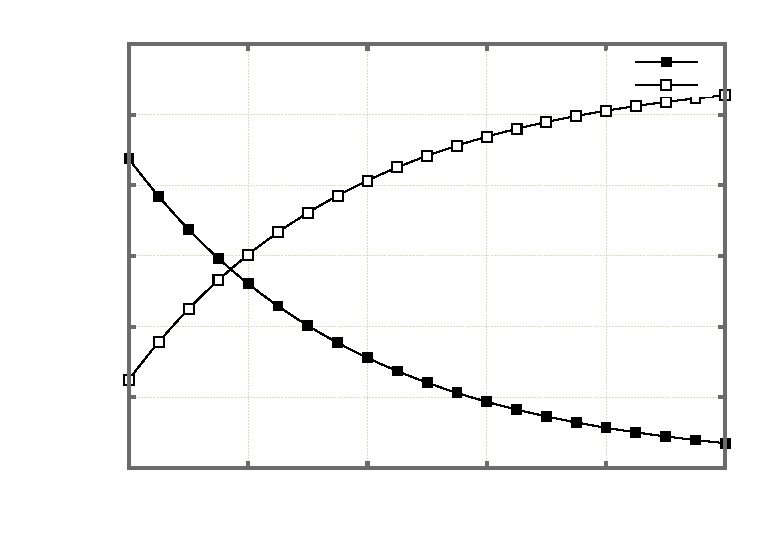
\includegraphics{twostate_2}}%
    \gplfronttext
  \end{picture}%
\endgroup
}
            \caption{Under asymmetric initial concentrations, a clear translation
            within the system is noticable. Otherwise the dynamics stay
            unaffected.}
            \label{fig:twostate_2}
         \end{minipage}
      \end{figure}

      As \cref{fig:twostate_lower_barrier} suggests, the convergence appears
      even quicker when the barrier is lowered. Comparison between
      \cref{fig:twostate_2} and \cref{fig:twostate_lower_barrier} also
      emphasises that the systems reaches its plateau at the same level, i.e. at
      the same fraction between $[A]$ and $[B]$, in both cases, independently of
      the barrier amplitude. 
      
      Our model also suggests that we, if we were to have a barrier height of
      $\Delta G^\ddagger_E = 65$~kJ/mol, our forward rate especially, would instead be given
      $k_+ = 15.7$, whereas $k_-$ increases proportionally, which explains the rapid convergence in
      \cref{fig:twostate_lower_barrier}.

      \begin{figure}[H]
         \centering
         \resizebox{.7\columnwidth}{!}{% GNUPLOT: LaTeX picture with Postscript
\begingroup
  \makeatletter
  \providecommand\color[2][]{%
    \GenericError{(gnuplot) \space\space\space\@spaces}{%
      Package color not loaded in conjunction with
      terminal option `colourtext'%
    }{See the gnuplot documentation for explanation.%
    }{Either use 'blacktext' in gnuplot or load the package
      color.sty in LaTeX.}%
    \renewcommand\color[2][]{}%
  }%
  \providecommand\includegraphics[2][]{%
    \GenericError{(gnuplot) \space\space\space\@spaces}{%
      Package graphicx or graphics not loaded%
    }{See the gnuplot documentation for explanation.%
    }{The gnuplot epslatex terminal needs graphicx.sty or graphics.sty.}%
    \renewcommand\includegraphics[2][]{}%
  }%
  \providecommand\rotatebox[2]{#2}%
  \@ifundefined{ifGPcolor}{%
    \newif\ifGPcolor
    \GPcolorfalse
  }{}%
  \@ifundefined{ifGPblacktext}{%
    \newif\ifGPblacktext
    \GPblacktexttrue
  }{}%
  % define a \g@addto@macro without @ in the name:
  \let\gplgaddtomacro\g@addto@macro
  % define empty templates for all commands taking text:
  \gdef\gplbacktext{}%
  \gdef\gplfronttext{}%
  \makeatother
  \ifGPblacktext
    % no textcolor at all
    \def\colorrgb#1{}%
    \def\colorgray#1{}%
  \else
    % gray or color?
    \ifGPcolor
      \def\colorrgb#1{\color[rgb]{#1}}%
      \def\colorgray#1{\color[gray]{#1}}%
      \expandafter\def\csname LTw\endcsname{\color{white}}%
      \expandafter\def\csname LTb\endcsname{\color{black}}%
      \expandafter\def\csname LTa\endcsname{\color{black}}%
      \expandafter\def\csname LT0\endcsname{\color[rgb]{1,0,0}}%
      \expandafter\def\csname LT1\endcsname{\color[rgb]{0,1,0}}%
      \expandafter\def\csname LT2\endcsname{\color[rgb]{0,0,1}}%
      \expandafter\def\csname LT3\endcsname{\color[rgb]{1,0,1}}%
      \expandafter\def\csname LT4\endcsname{\color[rgb]{0,1,1}}%
      \expandafter\def\csname LT5\endcsname{\color[rgb]{1,1,0}}%
      \expandafter\def\csname LT6\endcsname{\color[rgb]{0,0,0}}%
      \expandafter\def\csname LT7\endcsname{\color[rgb]{1,0.3,0}}%
      \expandafter\def\csname LT8\endcsname{\color[rgb]{0.5,0.5,0.5}}%
    \else
      % gray
      \def\colorrgb#1{\color{black}}%
      \def\colorgray#1{\color[gray]{#1}}%
      \expandafter\def\csname LTw\endcsname{\color{white}}%
      \expandafter\def\csname LTb\endcsname{\color{black}}%
      \expandafter\def\csname LTa\endcsname{\color{black}}%
      \expandafter\def\csname LT0\endcsname{\color{black}}%
      \expandafter\def\csname LT1\endcsname{\color{black}}%
      \expandafter\def\csname LT2\endcsname{\color{black}}%
      \expandafter\def\csname LT3\endcsname{\color{black}}%
      \expandafter\def\csname LT4\endcsname{\color{black}}%
      \expandafter\def\csname LT5\endcsname{\color{black}}%
      \expandafter\def\csname LT6\endcsname{\color{black}}%
      \expandafter\def\csname LT7\endcsname{\color{black}}%
      \expandafter\def\csname LT8\endcsname{\color{black}}%
    \fi
  \fi
  \setlength{\unitlength}{0.0500bp}%
  \begin{picture}(7200.00,5040.00)%
    \gplgaddtomacro\gplbacktext{%
      \colorrgb{0.42,0.42,0.42}%
      \put(946,704){\makebox(0,0)[r]{\strut{}0.00}}%
      \colorrgb{0.42,0.42,0.42}%
      \put(946,1518){\makebox(0,0)[r]{\strut{}0.10}}%
      \colorrgb{0.42,0.42,0.42}%
      \put(946,2332){\makebox(0,0)[r]{\strut{}0.20}}%
      \colorrgb{0.42,0.42,0.42}%
      \put(946,3147){\makebox(0,0)[r]{\strut{}0.30}}%
      \colorrgb{0.42,0.42,0.42}%
      \put(946,3961){\makebox(0,0)[r]{\strut{}0.40}}%
      \colorrgb{0.42,0.42,0.42}%
      \put(946,4775){\makebox(0,0)[r]{\strut{}0.50}}%
      \colorrgb{0.42,0.42,0.42}%
      \put(1078,484){\makebox(0,0){\strut{} 0}}%
      \colorrgb{0.42,0.42,0.42}%
      \put(2223,484){\makebox(0,0){\strut{} 2}}%
      \colorrgb{0.42,0.42,0.42}%
      \put(3368,484){\makebox(0,0){\strut{} 4}}%
      \colorrgb{0.42,0.42,0.42}%
      \put(4513,484){\makebox(0,0){\strut{} 6}}%
      \colorrgb{0.42,0.42,0.42}%
      \put(5658,484){\makebox(0,0){\strut{} 8}}%
      \colorrgb{0.42,0.42,0.42}%
      \put(6803,484){\makebox(0,0){\strut{} 10}}%
      \colorrgb{0.42,0.42,0.42}%
      \put(176,2739){\rotatebox{-270}{\makebox(0,0){\strut{}Concentration}}}%
      \colorrgb{0.42,0.42,0.42}%
      \put(3940,154){\makebox(0,0){\strut{}Time}}%
      \colorrgb{0.42,0.42,0.42}%
      \put(3940,4665){\makebox(0,0){\strut{}}}%
    }%
    \gplgaddtomacro\gplfronttext{%
      \csname LTb\endcsname%
      \put(5804,4602){\makebox(0,0)[r]{\strut{}A}}%
      \csname LTb\endcsname%
      \put(5804,4382){\makebox(0,0)[r]{\strut{}B}}%
    }%
    \gplbacktext
    \put(0,0){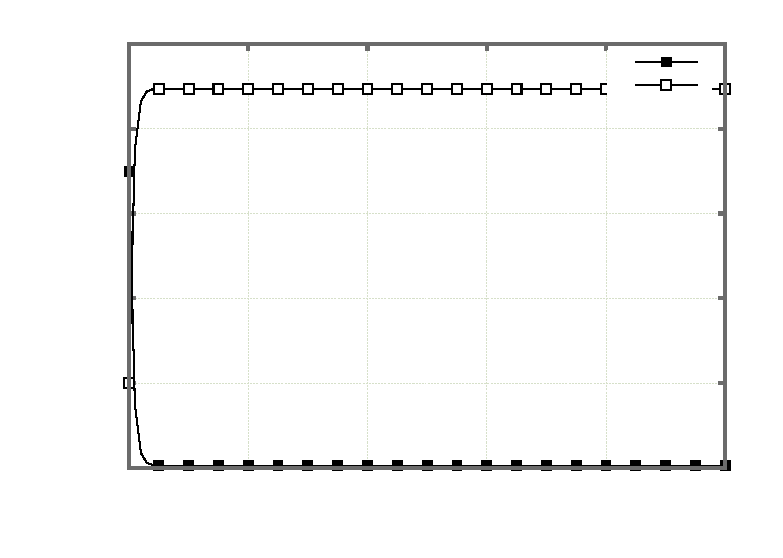
\includegraphics{twostate_lower_barrier}}%
    \gplfronttext
  \end{picture}%
\endgroup
}
         \caption{When the barrier is decreased in amplitude, the foremost
         consequence is that the rate from state $A \rightarrow B$ is increased
         multiply, whereas the rate $B\rightarrow A$ only increases slightly.}
         \label{fig:twostate_lower_barrier}
      \end{figure}

      Introducing our catlysed reaction scheme, the introduction of the enzyme
      $E$ is apparent in both \cref{fig:enzyme_low} where $[E]$ is low, and
      \cref{fig:enzyme_high} where $[E]$ is high, as also the dynamics
      emphasise. 

      \begin{figure}[H]
         \vspace*{1cm}
         \hspace*{-2cm}
         \centering
         \begin{minipage}[t]{.6\textwidth}		
            \vspace{0pt}
            \centering
            \resizebox{\columnwidth}{!}{% GNUPLOT: LaTeX picture with Postscript
\begingroup
  \makeatletter
  \providecommand\color[2][]{%
    \GenericError{(gnuplot) \space\space\space\@spaces}{%
      Package color not loaded in conjunction with
      terminal option `colourtext'%
    }{See the gnuplot documentation for explanation.%
    }{Either use 'blacktext' in gnuplot or load the package
      color.sty in LaTeX.}%
    \renewcommand\color[2][]{}%
  }%
  \providecommand\includegraphics[2][]{%
    \GenericError{(gnuplot) \space\space\space\@spaces}{%
      Package graphicx or graphics not loaded%
    }{See the gnuplot documentation for explanation.%
    }{The gnuplot epslatex terminal needs graphicx.sty or graphics.sty.}%
    \renewcommand\includegraphics[2][]{}%
  }%
  \providecommand\rotatebox[2]{#2}%
  \@ifundefined{ifGPcolor}{%
    \newif\ifGPcolor
    \GPcolorfalse
  }{}%
  \@ifundefined{ifGPblacktext}{%
    \newif\ifGPblacktext
    \GPblacktexttrue
  }{}%
  % define a \g@addto@macro without @ in the name:
  \let\gplgaddtomacro\g@addto@macro
  % define empty templates for all commands taking text:
  \gdef\gplbacktext{}%
  \gdef\gplfronttext{}%
  \makeatother
  \ifGPblacktext
    % no textcolor at all
    \def\colorrgb#1{}%
    \def\colorgray#1{}%
  \else
    % gray or color?
    \ifGPcolor
      \def\colorrgb#1{\color[rgb]{#1}}%
      \def\colorgray#1{\color[gray]{#1}}%
      \expandafter\def\csname LTw\endcsname{\color{white}}%
      \expandafter\def\csname LTb\endcsname{\color{black}}%
      \expandafter\def\csname LTa\endcsname{\color{black}}%
      \expandafter\def\csname LT0\endcsname{\color[rgb]{1,0,0}}%
      \expandafter\def\csname LT1\endcsname{\color[rgb]{0,1,0}}%
      \expandafter\def\csname LT2\endcsname{\color[rgb]{0,0,1}}%
      \expandafter\def\csname LT3\endcsname{\color[rgb]{1,0,1}}%
      \expandafter\def\csname LT4\endcsname{\color[rgb]{0,1,1}}%
      \expandafter\def\csname LT5\endcsname{\color[rgb]{1,1,0}}%
      \expandafter\def\csname LT6\endcsname{\color[rgb]{0,0,0}}%
      \expandafter\def\csname LT7\endcsname{\color[rgb]{1,0.3,0}}%
      \expandafter\def\csname LT8\endcsname{\color[rgb]{0.5,0.5,0.5}}%
    \else
      % gray
      \def\colorrgb#1{\color{black}}%
      \def\colorgray#1{\color[gray]{#1}}%
      \expandafter\def\csname LTw\endcsname{\color{white}}%
      \expandafter\def\csname LTb\endcsname{\color{black}}%
      \expandafter\def\csname LTa\endcsname{\color{black}}%
      \expandafter\def\csname LT0\endcsname{\color{black}}%
      \expandafter\def\csname LT1\endcsname{\color{black}}%
      \expandafter\def\csname LT2\endcsname{\color{black}}%
      \expandafter\def\csname LT3\endcsname{\color{black}}%
      \expandafter\def\csname LT4\endcsname{\color{black}}%
      \expandafter\def\csname LT5\endcsname{\color{black}}%
      \expandafter\def\csname LT6\endcsname{\color{black}}%
      \expandafter\def\csname LT7\endcsname{\color{black}}%
      \expandafter\def\csname LT8\endcsname{\color{black}}%
    \fi
  \fi
  \setlength{\unitlength}{0.0500bp}%
  \begin{picture}(7200.00,5040.00)%
    \gplgaddtomacro\gplbacktext{%
      \colorrgb{0.42,0.42,0.42}%
      \put(946,704){\makebox(0,0)[r]{\strut{}0.00}}%
      \colorrgb{0.42,0.42,0.42}%
      \put(946,1722){\makebox(0,0)[r]{\strut{}0.10}}%
      \colorrgb{0.42,0.42,0.42}%
      \put(946,2740){\makebox(0,0)[r]{\strut{}0.20}}%
      \colorrgb{0.42,0.42,0.42}%
      \put(946,3757){\makebox(0,0)[r]{\strut{}0.30}}%
      \colorrgb{0.42,0.42,0.42}%
      \put(946,4775){\makebox(0,0)[r]{\strut{}0.40}}%
      \colorrgb{0.42,0.42,0.42}%
      \put(1078,484){\makebox(0,0){\strut{} 0}}%
      \colorrgb{0.42,0.42,0.42}%
      \put(2223,484){\makebox(0,0){\strut{} 2}}%
      \colorrgb{0.42,0.42,0.42}%
      \put(3368,484){\makebox(0,0){\strut{} 4}}%
      \colorrgb{0.42,0.42,0.42}%
      \put(4513,484){\makebox(0,0){\strut{} 6}}%
      \colorrgb{0.42,0.42,0.42}%
      \put(5658,484){\makebox(0,0){\strut{} 8}}%
      \colorrgb{0.42,0.42,0.42}%
      \put(6803,484){\makebox(0,0){\strut{} 10}}%
      \colorrgb{0.42,0.42,0.42}%
      \put(176,2739){\rotatebox{-270}{\makebox(0,0){\strut{}Concentration}}}%
      \colorrgb{0.42,0.42,0.42}%
      \put(3940,154){\makebox(0,0){\strut{}Time}}%
      \colorrgb{0.42,0.42,0.42}%
      \put(3940,4665){\makebox(0,0){\strut{}}}%
    }%
    \gplgaddtomacro\gplfronttext{%
      \csname LTb\endcsname%
      \put(5804,4602){\makebox(0,0)[r]{\strut{}A}}%
      \csname LTb\endcsname%
      \put(5804,4382){\makebox(0,0)[r]{\strut{}B}}%
      \csname LTb\endcsname%
      \put(5804,4162){\makebox(0,0)[r]{\strut{}E}}%
    }%
    \gplbacktext
    \put(0,0){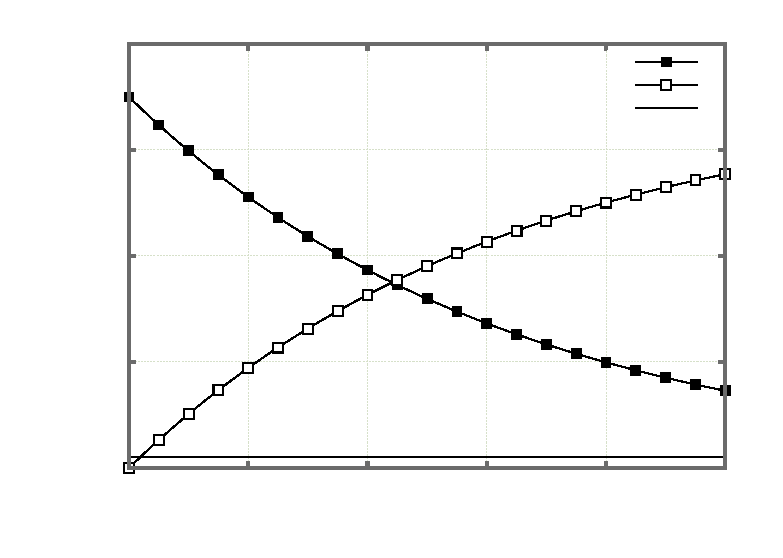
\includegraphics{enzyme_low}}%
    \gplfronttext
  \end{picture}%
\endgroup
}
            \caption{Catalysed system. Enzyme concentration low.}
            \label{fig:enzyme_low}
         \end{minipage}~\hspace*{1em}
         \begin{minipage}[t]{.6\textwidth}		
            \vspace{0pt}
            \centering
            \resizebox{\columnwidth}{!}{% GNUPLOT: LaTeX picture with Postscript
\begingroup
  \makeatletter
  \providecommand\color[2][]{%
    \GenericError{(gnuplot) \space\space\space\@spaces}{%
      Package color not loaded in conjunction with
      terminal option `colourtext'%
    }{See the gnuplot documentation for explanation.%
    }{Either use 'blacktext' in gnuplot or load the package
      color.sty in LaTeX.}%
    \renewcommand\color[2][]{}%
  }%
  \providecommand\includegraphics[2][]{%
    \GenericError{(gnuplot) \space\space\space\@spaces}{%
      Package graphicx or graphics not loaded%
    }{See the gnuplot documentation for explanation.%
    }{The gnuplot epslatex terminal needs graphicx.sty or graphics.sty.}%
    \renewcommand\includegraphics[2][]{}%
  }%
  \providecommand\rotatebox[2]{#2}%
  \@ifundefined{ifGPcolor}{%
    \newif\ifGPcolor
    \GPcolorfalse
  }{}%
  \@ifundefined{ifGPblacktext}{%
    \newif\ifGPblacktext
    \GPblacktexttrue
  }{}%
  % define a \g@addto@macro without @ in the name:
  \let\gplgaddtomacro\g@addto@macro
  % define empty templates for all commands taking text:
  \gdef\gplbacktext{}%
  \gdef\gplfronttext{}%
  \makeatother
  \ifGPblacktext
    % no textcolor at all
    \def\colorrgb#1{}%
    \def\colorgray#1{}%
  \else
    % gray or color?
    \ifGPcolor
      \def\colorrgb#1{\color[rgb]{#1}}%
      \def\colorgray#1{\color[gray]{#1}}%
      \expandafter\def\csname LTw\endcsname{\color{white}}%
      \expandafter\def\csname LTb\endcsname{\color{black}}%
      \expandafter\def\csname LTa\endcsname{\color{black}}%
      \expandafter\def\csname LT0\endcsname{\color[rgb]{1,0,0}}%
      \expandafter\def\csname LT1\endcsname{\color[rgb]{0,1,0}}%
      \expandafter\def\csname LT2\endcsname{\color[rgb]{0,0,1}}%
      \expandafter\def\csname LT3\endcsname{\color[rgb]{1,0,1}}%
      \expandafter\def\csname LT4\endcsname{\color[rgb]{0,1,1}}%
      \expandafter\def\csname LT5\endcsname{\color[rgb]{1,1,0}}%
      \expandafter\def\csname LT6\endcsname{\color[rgb]{0,0,0}}%
      \expandafter\def\csname LT7\endcsname{\color[rgb]{1,0.3,0}}%
      \expandafter\def\csname LT8\endcsname{\color[rgb]{0.5,0.5,0.5}}%
    \else
      % gray
      \def\colorrgb#1{\color{black}}%
      \def\colorgray#1{\color[gray]{#1}}%
      \expandafter\def\csname LTw\endcsname{\color{white}}%
      \expandafter\def\csname LTb\endcsname{\color{black}}%
      \expandafter\def\csname LTa\endcsname{\color{black}}%
      \expandafter\def\csname LT0\endcsname{\color{black}}%
      \expandafter\def\csname LT1\endcsname{\color{black}}%
      \expandafter\def\csname LT2\endcsname{\color{black}}%
      \expandafter\def\csname LT3\endcsname{\color{black}}%
      \expandafter\def\csname LT4\endcsname{\color{black}}%
      \expandafter\def\csname LT5\endcsname{\color{black}}%
      \expandafter\def\csname LT6\endcsname{\color{black}}%
      \expandafter\def\csname LT7\endcsname{\color{black}}%
      \expandafter\def\csname LT8\endcsname{\color{black}}%
    \fi
  \fi
  \setlength{\unitlength}{0.0500bp}%
  \begin{picture}(7200.00,5040.00)%
    \gplgaddtomacro\gplbacktext{%
      \colorrgb{0.42,0.42,0.42}%
      \put(946,704){\makebox(0,0)[r]{\strut{}0.00}}%
      \colorrgb{0.42,0.42,0.42}%
      \put(946,1722){\makebox(0,0)[r]{\strut{}0.10}}%
      \colorrgb{0.42,0.42,0.42}%
      \put(946,2740){\makebox(0,0)[r]{\strut{}0.20}}%
      \colorrgb{0.42,0.42,0.42}%
      \put(946,3757){\makebox(0,0)[r]{\strut{}0.30}}%
      \colorrgb{0.42,0.42,0.42}%
      \put(946,4775){\makebox(0,0)[r]{\strut{}0.40}}%
      \colorrgb{0.42,0.42,0.42}%
      \put(1078,484){\makebox(0,0){\strut{} 0}}%
      \colorrgb{0.42,0.42,0.42}%
      \put(2223,484){\makebox(0,0){\strut{} 2}}%
      \colorrgb{0.42,0.42,0.42}%
      \put(3368,484){\makebox(0,0){\strut{} 4}}%
      \colorrgb{0.42,0.42,0.42}%
      \put(4513,484){\makebox(0,0){\strut{} 6}}%
      \colorrgb{0.42,0.42,0.42}%
      \put(5658,484){\makebox(0,0){\strut{} 8}}%
      \colorrgb{0.42,0.42,0.42}%
      \put(6803,484){\makebox(0,0){\strut{} 10}}%
      \colorrgb{0.42,0.42,0.42}%
      \put(176,2739){\rotatebox{-270}{\makebox(0,0){\strut{}Concentration}}}%
      \colorrgb{0.42,0.42,0.42}%
      \put(3940,154){\makebox(0,0){\strut{}Time}}%
      \colorrgb{0.42,0.42,0.42}%
      \put(3940,4665){\makebox(0,0){\strut{}}}%
    }%
    \gplgaddtomacro\gplfronttext{%
      \csname LTb\endcsname%
      \put(5804,4602){\makebox(0,0)[r]{\strut{}A}}%
      \csname LTb\endcsname%
      \put(5804,4382){\makebox(0,0)[r]{\strut{}B}}%
      \csname LTb\endcsname%
      \put(5804,4162){\makebox(0,0)[r]{\strut{}E}}%
    }%
    \gplbacktext
    \put(0,0){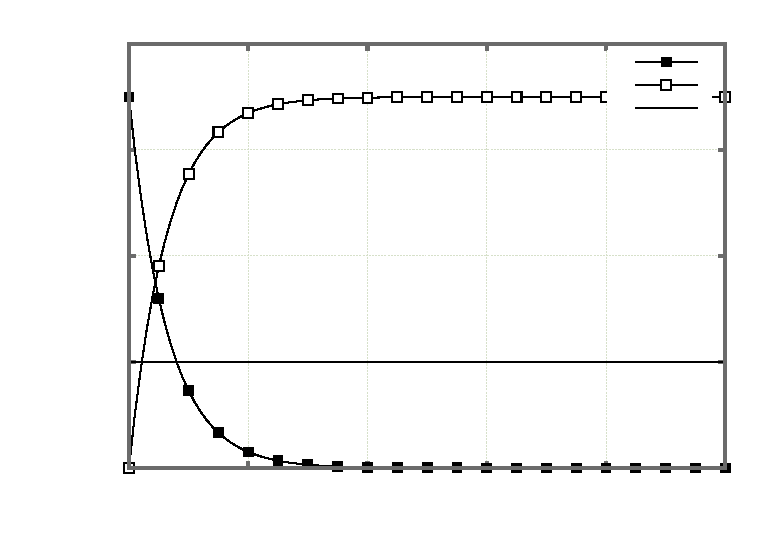
\includegraphics{enzyme_high}}%
    \gplfronttext
  \end{picture}%
\endgroup
}
            \caption{Catalysed system with high, constant concentration of
               enzyme. Note the increased convergence compared to the system
               with low concentration of enzyme.}
            \label{fig:enzyme_high}
         \end{minipage}
      \end{figure}

      When instead applying the Michaelis-Menten equation in our model, we can
      easily attain the same behaviour as without the introduced in-between
      step. We do however see that when the concentration of substance $[A]$ is 
      increased so that the enzymes are in clear minority, we instead get the 
      behaviour visible in \cref{fig:mm}, i.e. a linear increase in the
      concentration of $B$, until the point where the concentration of
      $A$ no longer is sufficient to uphold this behaviour. As apparent, we do
      not get our earlier assumed infinite rate, as a fraction of the enzymes
      now are bound to the complex substance $AE$, which bottlenecks this
      behaviour by limiting the amount of $E$ available for more complexes to be
      produced. The linearity ought thereby be inherent to the rate $k_+$, which
      also is the case.

      \begin{figure}[H]
         \centering
         \resizebox{.7\columnwidth}{!}{% GNUPLOT: LaTeX picture with Postscript
\begingroup
  \makeatletter
  \providecommand\color[2][]{%
    \GenericError{(gnuplot) \space\space\space\@spaces}{%
      Package color not loaded in conjunction with
      terminal option `colourtext'%
    }{See the gnuplot documentation for explanation.%
    }{Either use 'blacktext' in gnuplot or load the package
      color.sty in LaTeX.}%
    \renewcommand\color[2][]{}%
  }%
  \providecommand\includegraphics[2][]{%
    \GenericError{(gnuplot) \space\space\space\@spaces}{%
      Package graphicx or graphics not loaded%
    }{See the gnuplot documentation for explanation.%
    }{The gnuplot epslatex terminal needs graphicx.sty or graphics.sty.}%
    \renewcommand\includegraphics[2][]{}%
  }%
  \providecommand\rotatebox[2]{#2}%
  \@ifundefined{ifGPcolor}{%
    \newif\ifGPcolor
    \GPcolorfalse
  }{}%
  \@ifundefined{ifGPblacktext}{%
    \newif\ifGPblacktext
    \GPblacktexttrue
  }{}%
  % define a \g@addto@macro without @ in the name:
  \let\gplgaddtomacro\g@addto@macro
  % define empty templates for all commands taking text:
  \gdef\gplbacktext{}%
  \gdef\gplfronttext{}%
  \makeatother
  \ifGPblacktext
    % no textcolor at all
    \def\colorrgb#1{}%
    \def\colorgray#1{}%
  \else
    % gray or color?
    \ifGPcolor
      \def\colorrgb#1{\color[rgb]{#1}}%
      \def\colorgray#1{\color[gray]{#1}}%
      \expandafter\def\csname LTw\endcsname{\color{white}}%
      \expandafter\def\csname LTb\endcsname{\color{black}}%
      \expandafter\def\csname LTa\endcsname{\color{black}}%
      \expandafter\def\csname LT0\endcsname{\color[rgb]{1,0,0}}%
      \expandafter\def\csname LT1\endcsname{\color[rgb]{0,1,0}}%
      \expandafter\def\csname LT2\endcsname{\color[rgb]{0,0,1}}%
      \expandafter\def\csname LT3\endcsname{\color[rgb]{1,0,1}}%
      \expandafter\def\csname LT4\endcsname{\color[rgb]{0,1,1}}%
      \expandafter\def\csname LT5\endcsname{\color[rgb]{1,1,0}}%
      \expandafter\def\csname LT6\endcsname{\color[rgb]{0,0,0}}%
      \expandafter\def\csname LT7\endcsname{\color[rgb]{1,0.3,0}}%
      \expandafter\def\csname LT8\endcsname{\color[rgb]{0.5,0.5,0.5}}%
    \else
      % gray
      \def\colorrgb#1{\color{black}}%
      \def\colorgray#1{\color[gray]{#1}}%
      \expandafter\def\csname LTw\endcsname{\color{white}}%
      \expandafter\def\csname LTb\endcsname{\color{black}}%
      \expandafter\def\csname LTa\endcsname{\color{black}}%
      \expandafter\def\csname LT0\endcsname{\color{black}}%
      \expandafter\def\csname LT1\endcsname{\color{black}}%
      \expandafter\def\csname LT2\endcsname{\color{black}}%
      \expandafter\def\csname LT3\endcsname{\color{black}}%
      \expandafter\def\csname LT4\endcsname{\color{black}}%
      \expandafter\def\csname LT5\endcsname{\color{black}}%
      \expandafter\def\csname LT6\endcsname{\color{black}}%
      \expandafter\def\csname LT7\endcsname{\color{black}}%
      \expandafter\def\csname LT8\endcsname{\color{black}}%
    \fi
  \fi
  \setlength{\unitlength}{0.0500bp}%
  \begin{picture}(7200.00,5040.00)%
    \gplgaddtomacro\gplbacktext{%
      \colorrgb{0.42,0.42,0.42}%
      \put(946,704){\makebox(0,0)[r]{\strut{}0}}%
      \colorrgb{0.42,0.42,0.42}%
      \put(946,1383){\makebox(0,0)[r]{\strut{}200}}%
      \colorrgb{0.42,0.42,0.42}%
      \put(946,2061){\makebox(0,0)[r]{\strut{}400}}%
      \colorrgb{0.42,0.42,0.42}%
      \put(946,2740){\makebox(0,0)[r]{\strut{}600}}%
      \colorrgb{0.42,0.42,0.42}%
      \put(946,3418){\makebox(0,0)[r]{\strut{}800}}%
      \colorrgb{0.42,0.42,0.42}%
      \put(946,4097){\makebox(0,0)[r]{\strut{}1000}}%
      \colorrgb{0.42,0.42,0.42}%
      \put(946,4775){\makebox(0,0)[r]{\strut{}1200}}%
      \colorrgb{0.42,0.42,0.42}%
      \put(1078,484){\makebox(0,0){\strut{} 0}}%
      \colorrgb{0.42,0.42,0.42}%
      \put(2223,484){\makebox(0,0){\strut{} 20}}%
      \colorrgb{0.42,0.42,0.42}%
      \put(3368,484){\makebox(0,0){\strut{} 40}}%
      \colorrgb{0.42,0.42,0.42}%
      \put(4513,484){\makebox(0,0){\strut{} 60}}%
      \colorrgb{0.42,0.42,0.42}%
      \put(5658,484){\makebox(0,0){\strut{} 80}}%
      \colorrgb{0.42,0.42,0.42}%
      \put(6803,484){\makebox(0,0){\strut{} 100}}%
      \colorrgb{0.42,0.42,0.42}%
      \put(176,2739){\rotatebox{-270}{\makebox(0,0){\strut{}Concentration}}}%
      \colorrgb{0.42,0.42,0.42}%
      \put(3940,154){\makebox(0,0){\strut{}Time}}%
      \colorrgb{0.42,0.42,0.42}%
      \put(3940,4665){\makebox(0,0){\strut{}}}%
    }%
    \gplgaddtomacro\gplfronttext{%
      \csname LTb\endcsname%
      \put(5804,4602){\makebox(0,0)[r]{\strut{}A}}%
      \csname LTb\endcsname%
      \put(5804,4382){\makebox(0,0)[r]{\strut{}B}}%
    }%
    \gplbacktext
    \put(0,0){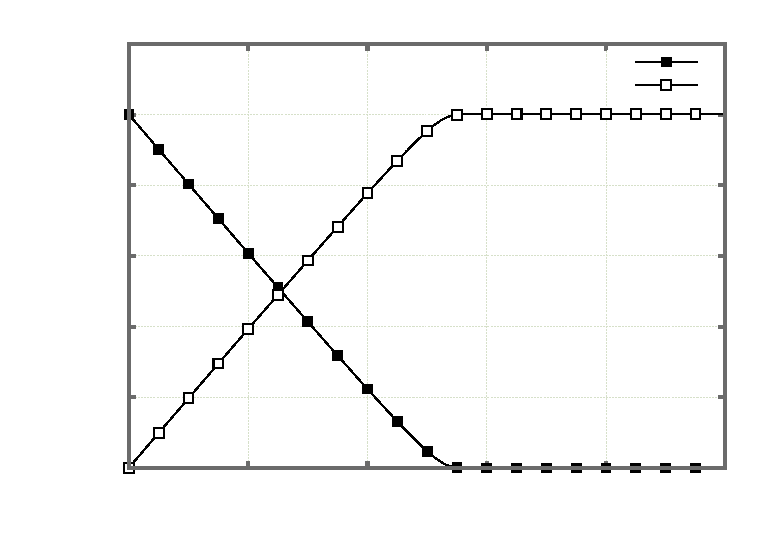
\includegraphics{mm}}%
    \gplfronttext
  \end{picture}%
\endgroup
}
         \caption{Concentration of $[A]$ in heavy supply, whereas the total
            amount of enzymes is constant. We achieve a linear behaviour until
            the concentration of $A$ is insufficient. }
         \label{fig:mm}
      \end{figure}

      \begin{figure}[H]
         \centering
         \resizebox{.7\columnwidth}{!}{% GNUPLOT: LaTeX picture with Postscript
\begingroup
  \makeatletter
  \providecommand\color[2][]{%
    \GenericError{(gnuplot) \space\space\space\@spaces}{%
      Package color not loaded in conjunction with
      terminal option `colourtext'%
    }{See the gnuplot documentation for explanation.%
    }{Either use 'blacktext' in gnuplot or load the package
      color.sty in LaTeX.}%
    \renewcommand\color[2][]{}%
  }%
  \providecommand\includegraphics[2][]{%
    \GenericError{(gnuplot) \space\space\space\@spaces}{%
      Package graphicx or graphics not loaded%
    }{See the gnuplot documentation for explanation.%
    }{The gnuplot epslatex terminal needs graphicx.sty or graphics.sty.}%
    \renewcommand\includegraphics[2][]{}%
  }%
  \providecommand\rotatebox[2]{#2}%
  \@ifundefined{ifGPcolor}{%
    \newif\ifGPcolor
    \GPcolortrue
  }{}%
  \@ifundefined{ifGPblacktext}{%
    \newif\ifGPblacktext
    \GPblacktexttrue
  }{}%
  % define a \g@addto@macro without @ in the name:
  \let\gplgaddtomacro\g@addto@macro
  % define empty templates for all commands taking text:
  \gdef\gplbacktext{}%
  \gdef\gplfronttext{}%
  \makeatother
  \ifGPblacktext
    % no textcolor at all
    \def\colorrgb#1{}%
    \def\colorgray#1{}%
  \else
    % gray or color?
    \ifGPcolor
      \def\colorrgb#1{\color[rgb]{#1}}%
      \def\colorgray#1{\color[gray]{#1}}%
      \expandafter\def\csname LTw\endcsname{\color{white}}%
      \expandafter\def\csname LTb\endcsname{\color{black}}%
      \expandafter\def\csname LTa\endcsname{\color{black}}%
      \expandafter\def\csname LT0\endcsname{\color[rgb]{1,0,0}}%
      \expandafter\def\csname LT1\endcsname{\color[rgb]{0,1,0}}%
      \expandafter\def\csname LT2\endcsname{\color[rgb]{0,0,1}}%
      \expandafter\def\csname LT3\endcsname{\color[rgb]{1,0,1}}%
      \expandafter\def\csname LT4\endcsname{\color[rgb]{0,1,1}}%
      \expandafter\def\csname LT5\endcsname{\color[rgb]{1,1,0}}%
      \expandafter\def\csname LT6\endcsname{\color[rgb]{0,0,0}}%
      \expandafter\def\csname LT7\endcsname{\color[rgb]{1,0.3,0}}%
      \expandafter\def\csname LT8\endcsname{\color[rgb]{0.5,0.5,0.5}}%
    \else
      % gray
      \def\colorrgb#1{\color{black}}%
      \def\colorgray#1{\color[gray]{#1}}%
      \expandafter\def\csname LTw\endcsname{\color{white}}%
      \expandafter\def\csname LTb\endcsname{\color{black}}%
      \expandafter\def\csname LTa\endcsname{\color{black}}%
      \expandafter\def\csname LT0\endcsname{\color{black}}%
      \expandafter\def\csname LT1\endcsname{\color{black}}%
      \expandafter\def\csname LT2\endcsname{\color{black}}%
      \expandafter\def\csname LT3\endcsname{\color{black}}%
      \expandafter\def\csname LT4\endcsname{\color{black}}%
      \expandafter\def\csname LT5\endcsname{\color{black}}%
      \expandafter\def\csname LT6\endcsname{\color{black}}%
      \expandafter\def\csname LT7\endcsname{\color{black}}%
      \expandafter\def\csname LT8\endcsname{\color{black}}%
    \fi
  \fi
  \setlength{\unitlength}{0.0500bp}%
  \begin{picture}(7200.00,5040.00)%
    \gplgaddtomacro\gplbacktext{%
      \colorrgb{0.42,0.42,0.42}%
      \put(3600,4312){\makebox(0,0){\strut{}}}%
    }%
    \gplgaddtomacro\gplfronttext{%
      \colorrgb{0.42,0.42,0.42}%
      \put(1170,772){\makebox(0,0){\strut{} 0}}%
      \colorrgb{0.42,0.42,0.42}%
      \put(1656,772){\makebox(0,0){\strut{} 1}}%
      \colorrgb{0.42,0.42,0.42}%
      \put(2142,772){\makebox(0,0){\strut{} 2}}%
      \colorrgb{0.42,0.42,0.42}%
      \put(2628,772){\makebox(0,0){\strut{} 3}}%
      \colorrgb{0.42,0.42,0.42}%
      \put(3114,772){\makebox(0,0){\strut{} 4}}%
      \colorrgb{0.42,0.42,0.42}%
      \put(3600,772){\makebox(0,0){\strut{} 5}}%
      \colorrgb{0.42,0.42,0.42}%
      \put(4086,772){\makebox(0,0){\strut{} 6}}%
      \colorrgb{0.42,0.42,0.42}%
      \put(4572,772){\makebox(0,0){\strut{} 7}}%
      \colorrgb{0.42,0.42,0.42}%
      \put(5058,772){\makebox(0,0){\strut{} 8}}%
      \colorrgb{0.42,0.42,0.42}%
      \put(5544,772){\makebox(0,0){\strut{} 9}}%
      \colorrgb{0.42,0.42,0.42}%
      \put(6030,772){\makebox(0,0){\strut{} 10}}%
      \colorrgb{0.42,0.42,0.42}%
      \put(3600,442){\makebox(0,0){\strut{}Time}}%
      \colorrgb{0.42,0.42,0.42}%
      \put(998,1058){\makebox(0,0)[r]{\strut{} 0}}%
      \colorrgb{0.42,0.42,0.42}%
      \put(998,1383){\makebox(0,0)[r]{\strut{} 1}}%
      \colorrgb{0.42,0.42,0.42}%
      \put(998,1708){\makebox(0,0)[r]{\strut{} 2}}%
      \colorrgb{0.42,0.42,0.42}%
      \put(998,2033){\makebox(0,0)[r]{\strut{} 3}}%
      \colorrgb{0.42,0.42,0.42}%
      \put(998,2358){\makebox(0,0)[r]{\strut{} 4}}%
      \colorrgb{0.42,0.42,0.42}%
      \put(998,2682){\makebox(0,0)[r]{\strut{} 5}}%
      \colorrgb{0.42,0.42,0.42}%
      \put(998,3007){\makebox(0,0)[r]{\strut{} 6}}%
      \colorrgb{0.42,0.42,0.42}%
      \put(998,3332){\makebox(0,0)[r]{\strut{} 7}}%
      \colorrgb{0.42,0.42,0.42}%
      \put(998,3657){\makebox(0,0)[r]{\strut{} 8}}%
      \colorrgb{0.42,0.42,0.42}%
      \put(998,3982){\makebox(0,0)[r]{\strut{} 9}}%
      \colorrgb{0.42,0.42,0.42}%
      \put(668,2520){\rotatebox{-270}{\makebox(0,0){\strut{}Cell}}}%
      \colorrgb{0.42,0.42,0.42}%
      \put(6527,1058){\makebox(0,0)[l]{\strut{} 2}}%
      \colorrgb{0.42,0.42,0.42}%
      \put(6527,1423){\makebox(0,0)[l]{\strut{} 3}}%
      \colorrgb{0.42,0.42,0.42}%
      \put(6527,1789){\makebox(0,0)[l]{\strut{} 4}}%
      \colorrgb{0.42,0.42,0.42}%
      \put(6527,2154){\makebox(0,0)[l]{\strut{} 5}}%
      \colorrgb{0.42,0.42,0.42}%
      \put(6527,2520){\makebox(0,0)[l]{\strut{} 6}}%
      \colorrgb{0.42,0.42,0.42}%
      \put(6527,2885){\makebox(0,0)[l]{\strut{} 7}}%
      \colorrgb{0.42,0.42,0.42}%
      \put(6527,3251){\makebox(0,0)[l]{\strut{} 8}}%
      \colorrgb{0.42,0.42,0.42}%
      \put(6527,3616){\makebox(0,0)[l]{\strut{} 9}}%
      \colorrgb{0.42,0.42,0.42}%
      \put(6527,3982){\makebox(0,0)[l]{\strut{} 10}}%
    }%
    \gplbacktext
    \put(0,0){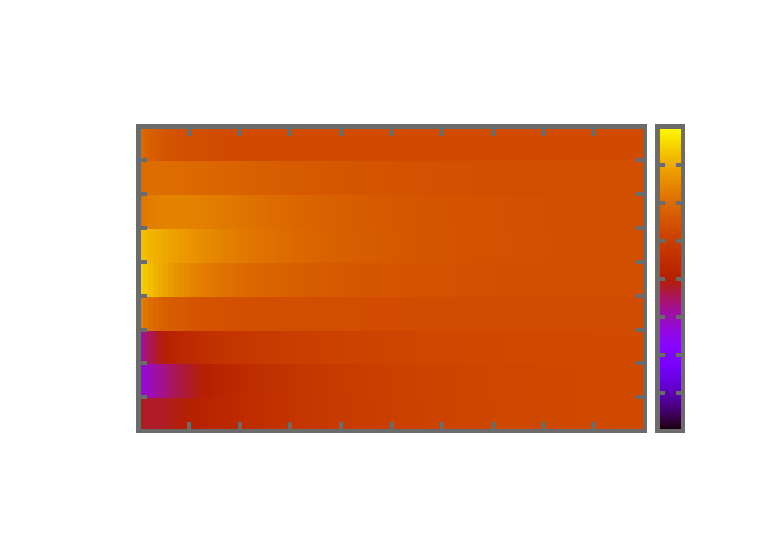
\includegraphics{diff}}%
    \gplfronttext
  \end{picture}%
\endgroup
}
         \caption{Simple diffusion network. Gradient corresponds to
         concentration, as in all following images.}
         \label{fig:diff}
      \end{figure}
   
      \Cref{fig:diff} displays the dynamics of a 10--cell system undergoing
      diffusion after all cells have been initialized with random initial
      concentrations. As in Nelson~\cite{nelson}, the effects of diffusion are
      clearly visible, as all cells trend towards a common, steady-state
      concentration.

      \begin{figure}[H]
         \vspace*{1cm}
         \hspace*{-2cm}
         \centering
         \begin{minipage}[t]{.6\textwidth}		
            \vspace{30pt}
            \centering
            \resizebox{\columnwidth}{!}{% GNUPLOT: LaTeX picture with Postscript
\begingroup
  \makeatletter
  \providecommand\color[2][]{%
    \GenericError{(gnuplot) \space\space\space\@spaces}{%
      Package color not loaded in conjunction with
      terminal option `colourtext'%
    }{See the gnuplot documentation for explanation.%
    }{Either use 'blacktext' in gnuplot or load the package
      color.sty in LaTeX.}%
    \renewcommand\color[2][]{}%
  }%
  \providecommand\includegraphics[2][]{%
    \GenericError{(gnuplot) \space\space\space\@spaces}{%
      Package graphicx or graphics not loaded%
    }{See the gnuplot documentation for explanation.%
    }{The gnuplot epslatex terminal needs graphicx.sty or graphics.sty.}%
    \renewcommand\includegraphics[2][]{}%
  }%
  \providecommand\rotatebox[2]{#2}%
  \@ifundefined{ifGPcolor}{%
    \newif\ifGPcolor
    \GPcolortrue
  }{}%
  \@ifundefined{ifGPblacktext}{%
    \newif\ifGPblacktext
    \GPblacktexttrue
  }{}%
  % define a \g@addto@macro without @ in the name:
  \let\gplgaddtomacro\g@addto@macro
  % define empty templates for all commands taking text:
  \gdef\gplbacktext{}%
  \gdef\gplfronttext{}%
  \makeatother
  \ifGPblacktext
    % no textcolor at all
    \def\colorrgb#1{}%
    \def\colorgray#1{}%
  \else
    % gray or color?
    \ifGPcolor
      \def\colorrgb#1{\color[rgb]{#1}}%
      \def\colorgray#1{\color[gray]{#1}}%
      \expandafter\def\csname LTw\endcsname{\color{white}}%
      \expandafter\def\csname LTb\endcsname{\color{black}}%
      \expandafter\def\csname LTa\endcsname{\color{black}}%
      \expandafter\def\csname LT0\endcsname{\color[rgb]{1,0,0}}%
      \expandafter\def\csname LT1\endcsname{\color[rgb]{0,1,0}}%
      \expandafter\def\csname LT2\endcsname{\color[rgb]{0,0,1}}%
      \expandafter\def\csname LT3\endcsname{\color[rgb]{1,0,1}}%
      \expandafter\def\csname LT4\endcsname{\color[rgb]{0,1,1}}%
      \expandafter\def\csname LT5\endcsname{\color[rgb]{1,1,0}}%
      \expandafter\def\csname LT6\endcsname{\color[rgb]{0,0,0}}%
      \expandafter\def\csname LT7\endcsname{\color[rgb]{1,0.3,0}}%
      \expandafter\def\csname LT8\endcsname{\color[rgb]{0.5,0.5,0.5}}%
    \else
      % gray
      \def\colorrgb#1{\color{black}}%
      \def\colorgray#1{\color[gray]{#1}}%
      \expandafter\def\csname LTw\endcsname{\color{white}}%
      \expandafter\def\csname LTb\endcsname{\color{black}}%
      \expandafter\def\csname LTa\endcsname{\color{black}}%
      \expandafter\def\csname LT0\endcsname{\color{black}}%
      \expandafter\def\csname LT1\endcsname{\color{black}}%
      \expandafter\def\csname LT2\endcsname{\color{black}}%
      \expandafter\def\csname LT3\endcsname{\color{black}}%
      \expandafter\def\csname LT4\endcsname{\color{black}}%
      \expandafter\def\csname LT5\endcsname{\color{black}}%
      \expandafter\def\csname LT6\endcsname{\color{black}}%
      \expandafter\def\csname LT7\endcsname{\color{black}}%
      \expandafter\def\csname LT8\endcsname{\color{black}}%
    \fi
  \fi
  \setlength{\unitlength}{0.0500bp}%
  \begin{picture}(7200.00,5040.00)%
    \gplgaddtomacro\gplbacktext{%
      \csname LTb\endcsname%
      \put(946,704){\makebox(0,0)[r]{\strut{} 0}}%
      \csname LTb\endcsname%
      \put(946,1383){\makebox(0,0)[r]{\strut{} 0.5}}%
      \csname LTb\endcsname%
      \put(946,2061){\makebox(0,0)[r]{\strut{} 1}}%
      \csname LTb\endcsname%
      \put(946,2740){\makebox(0,0)[r]{\strut{} 1.5}}%
      \csname LTb\endcsname%
      \put(946,3418){\makebox(0,0)[r]{\strut{} 2}}%
      \csname LTb\endcsname%
      \put(946,4097){\makebox(0,0)[r]{\strut{} 2.5}}%
      \csname LTb\endcsname%
      \put(946,4775){\makebox(0,0)[r]{\strut{} 3}}%
      \csname LTb\endcsname%
      \put(1078,484){\makebox(0,0){\strut{} 0}}%
      \csname LTb\endcsname%
      \put(1651,484){\makebox(0,0){\strut{} 2}}%
      \csname LTb\endcsname%
      \put(2223,484){\makebox(0,0){\strut{} 4}}%
      \csname LTb\endcsname%
      \put(2796,484){\makebox(0,0){\strut{} 6}}%
      \csname LTb\endcsname%
      \put(3368,484){\makebox(0,0){\strut{} 8}}%
      \csname LTb\endcsname%
      \put(3941,484){\makebox(0,0){\strut{} 10}}%
      \csname LTb\endcsname%
      \put(4513,484){\makebox(0,0){\strut{} 12}}%
      \csname LTb\endcsname%
      \put(5086,484){\makebox(0,0){\strut{} 14}}%
      \csname LTb\endcsname%
      \put(5658,484){\makebox(0,0){\strut{} 16}}%
      \csname LTb\endcsname%
      \put(6231,484){\makebox(0,0){\strut{} 18}}%
      \csname LTb\endcsname%
      \put(6803,484){\makebox(0,0){\strut{} 20}}%
      \put(176,2739){\rotatebox{-270}{\makebox(0,0){\strut{}Concentration}}}%
      \put(3940,154){\makebox(0,0){\strut{}Time}}%
    }%
    \gplgaddtomacro\gplfronttext{%
      \csname LTb\endcsname%
      \put(5816,4602){\makebox(0,0)[r]{\strut{}X}}%
      \csname LTb\endcsname%
      \put(5816,4382){\makebox(0,0)[r]{\strut{}Y}}%
    }%
    \gplbacktext
    \put(0,0){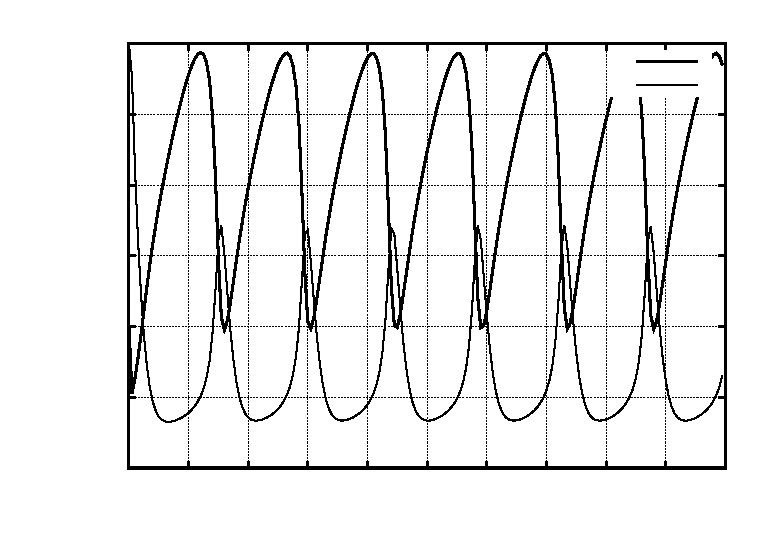
\includegraphics{brussel1}}%
    \gplfronttext
  \end{picture}%
\endgroup
}
            \caption{Concetration change for a single cell in the brusselator
            model. Rate value set $\mathcal{K} = \{2, 4, 6, 3\}$ for the
            different parameters respectively.}
            \label{fig:br1}
         \end{minipage}~\hspace*{1em}
         \begin{minipage}[t]{.6\textwidth}		
            \vspace{0pt}
            \centering
            \resizebox{1.2\columnwidth}{!}{% GNUPLOT: LaTeX picture with Postscript
\begingroup
  \makeatletter
  \providecommand\color[2][]{%
    \GenericError{(gnuplot) \space\space\space\@spaces}{%
      Package color not loaded in conjunction with
      terminal option `colourtext'%
    }{See the gnuplot documentation for explanation.%
    }{Either use 'blacktext' in gnuplot or load the package
      color.sty in LaTeX.}%
    \renewcommand\color[2][]{}%
  }%
  \providecommand\includegraphics[2][]{%
    \GenericError{(gnuplot) \space\space\space\@spaces}{%
      Package graphicx or graphics not loaded%
    }{See the gnuplot documentation for explanation.%
    }{The gnuplot epslatex terminal needs graphicx.sty or graphics.sty.}%
    \renewcommand\includegraphics[2][]{}%
  }%
  \providecommand\rotatebox[2]{#2}%
  \@ifundefined{ifGPcolor}{%
    \newif\ifGPcolor
    \GPcolortrue
  }{}%
  \@ifundefined{ifGPblacktext}{%
    \newif\ifGPblacktext
    \GPblacktexttrue
  }{}%
  % define a \g@addto@macro without @ in the name:
  \let\gplgaddtomacro\g@addto@macro
  % define empty templates for all commands taking text:
  \gdef\gplbacktext{}%
  \gdef\gplfronttext{}%
  \makeatother
  \ifGPblacktext
    % no textcolor at all
    \def\colorrgb#1{}%
    \def\colorgray#1{}%
  \else
    % gray or color?
    \ifGPcolor
      \def\colorrgb#1{\color[rgb]{#1}}%
      \def\colorgray#1{\color[gray]{#1}}%
      \expandafter\def\csname LTw\endcsname{\color{white}}%
      \expandafter\def\csname LTb\endcsname{\color{black}}%
      \expandafter\def\csname LTa\endcsname{\color{black}}%
      \expandafter\def\csname LT0\endcsname{\color[rgb]{1,0,0}}%
      \expandafter\def\csname LT1\endcsname{\color[rgb]{0,1,0}}%
      \expandafter\def\csname LT2\endcsname{\color[rgb]{0,0,1}}%
      \expandafter\def\csname LT3\endcsname{\color[rgb]{1,0,1}}%
      \expandafter\def\csname LT4\endcsname{\color[rgb]{0,1,1}}%
      \expandafter\def\csname LT5\endcsname{\color[rgb]{1,1,0}}%
      \expandafter\def\csname LT6\endcsname{\color[rgb]{0,0,0}}%
      \expandafter\def\csname LT7\endcsname{\color[rgb]{1,0.3,0}}%
      \expandafter\def\csname LT8\endcsname{\color[rgb]{0.5,0.5,0.5}}%
    \else
      % gray
      \def\colorrgb#1{\color{black}}%
      \def\colorgray#1{\color[gray]{#1}}%
      \expandafter\def\csname LTw\endcsname{\color{white}}%
      \expandafter\def\csname LTb\endcsname{\color{black}}%
      \expandafter\def\csname LTa\endcsname{\color{black}}%
      \expandafter\def\csname LT0\endcsname{\color{black}}%
      \expandafter\def\csname LT1\endcsname{\color{black}}%
      \expandafter\def\csname LT2\endcsname{\color{black}}%
      \expandafter\def\csname LT3\endcsname{\color{black}}%
      \expandafter\def\csname LT4\endcsname{\color{black}}%
      \expandafter\def\csname LT5\endcsname{\color{black}}%
      \expandafter\def\csname LT6\endcsname{\color{black}}%
      \expandafter\def\csname LT7\endcsname{\color{black}}%
      \expandafter\def\csname LT8\endcsname{\color{black}}%
    \fi
  \fi
  \setlength{\unitlength}{0.0500bp}%
  \begin{picture}(7200.00,5040.00)%
    \gplgaddtomacro\gplbacktext{%
      \colorrgb{0.42,0.42,0.42}%
      \put(3600,4312){\makebox(0,0){\strut{}}}%
    }%
    \gplgaddtomacro\gplfronttext{%
      \colorrgb{0.42,0.42,0.42}%
      \put(1170,772){\makebox(0,0){\strut{} 0}}%
      \colorrgb{0.42,0.42,0.42}%
      \put(1656,772){\makebox(0,0){\strut{} 2}}%
      \colorrgb{0.42,0.42,0.42}%
      \put(2142,772){\makebox(0,0){\strut{} 4}}%
      \colorrgb{0.42,0.42,0.42}%
      \put(2628,772){\makebox(0,0){\strut{} 6}}%
      \colorrgb{0.42,0.42,0.42}%
      \put(3114,772){\makebox(0,0){\strut{} 8}}%
      \colorrgb{0.42,0.42,0.42}%
      \put(3600,772){\makebox(0,0){\strut{} 10}}%
      \colorrgb{0.42,0.42,0.42}%
      \put(4086,772){\makebox(0,0){\strut{} 12}}%
      \colorrgb{0.42,0.42,0.42}%
      \put(4572,772){\makebox(0,0){\strut{} 14}}%
      \colorrgb{0.42,0.42,0.42}%
      \put(5058,772){\makebox(0,0){\strut{} 16}}%
      \colorrgb{0.42,0.42,0.42}%
      \put(5544,772){\makebox(0,0){\strut{} 18}}%
      \colorrgb{0.42,0.42,0.42}%
      \put(6030,772){\makebox(0,0){\strut{} 20}}%
      \colorrgb{0.42,0.42,0.42}%
      \put(3600,442){\makebox(0,0){\strut{}Time}}%
      \colorrgb{0.42,0.42,0.42}%
      \put(998,1058){\makebox(0,0)[r]{\strut{} 0}}%
      \colorrgb{0.42,0.42,0.42}%
      \put(998,1351){\makebox(0,0)[r]{\strut{} 10}}%
      \colorrgb{0.42,0.42,0.42}%
      \put(998,1643){\makebox(0,0)[r]{\strut{} 20}}%
      \colorrgb{0.42,0.42,0.42}%
      \put(998,1936){\makebox(0,0)[r]{\strut{} 30}}%
      \colorrgb{0.42,0.42,0.42}%
      \put(998,2228){\makebox(0,0)[r]{\strut{} 40}}%
      \colorrgb{0.42,0.42,0.42}%
      \put(998,2520){\makebox(0,0)[r]{\strut{} 50}}%
      \colorrgb{0.42,0.42,0.42}%
      \put(998,2812){\makebox(0,0)[r]{\strut{} 60}}%
      \colorrgb{0.42,0.42,0.42}%
      \put(998,3104){\makebox(0,0)[r]{\strut{} 70}}%
      \colorrgb{0.42,0.42,0.42}%
      \put(998,3397){\makebox(0,0)[r]{\strut{} 80}}%
      \colorrgb{0.42,0.42,0.42}%
      \put(998,3689){\makebox(0,0)[r]{\strut{} 90}}%
      \colorrgb{0.42,0.42,0.42}%
      \put(998,3982){\makebox(0,0)[r]{\strut{} 100}}%
      \colorrgb{0.42,0.42,0.42}%
      \put(404,2520){\rotatebox{-270}{\makebox(0,0){\strut{}Cell}}}%
      \colorrgb{0.42,0.42,0.42}%
      \put(6527,1058){\makebox(0,0)[l]{\strut{} 0}}%
      \colorrgb{0.42,0.42,0.42}%
      \put(6527,1382){\makebox(0,0)[l]{\strut{} 0.2}}%
      \colorrgb{0.42,0.42,0.42}%
      \put(6527,1707){\makebox(0,0)[l]{\strut{} 0.4}}%
      \colorrgb{0.42,0.42,0.42}%
      \put(6527,2032){\makebox(0,0)[l]{\strut{} 0.6}}%
      \colorrgb{0.42,0.42,0.42}%
      \put(6527,2357){\makebox(0,0)[l]{\strut{} 0.8}}%
      \colorrgb{0.42,0.42,0.42}%
      \put(6527,2682){\makebox(0,0)[l]{\strut{} 1}}%
      \colorrgb{0.42,0.42,0.42}%
      \put(6527,3007){\makebox(0,0)[l]{\strut{} 1.2}}%
      \colorrgb{0.42,0.42,0.42}%
      \put(6527,3332){\makebox(0,0)[l]{\strut{} 1.4}}%
      \colorrgb{0.42,0.42,0.42}%
      \put(6527,3657){\makebox(0,0)[l]{\strut{} 1.6}}%
      \colorrgb{0.42,0.42,0.42}%
      \put(6527,3981){\makebox(0,0)[l]{\strut{} 1.8}}%
    }%
    \gplbacktext
    \put(0,0){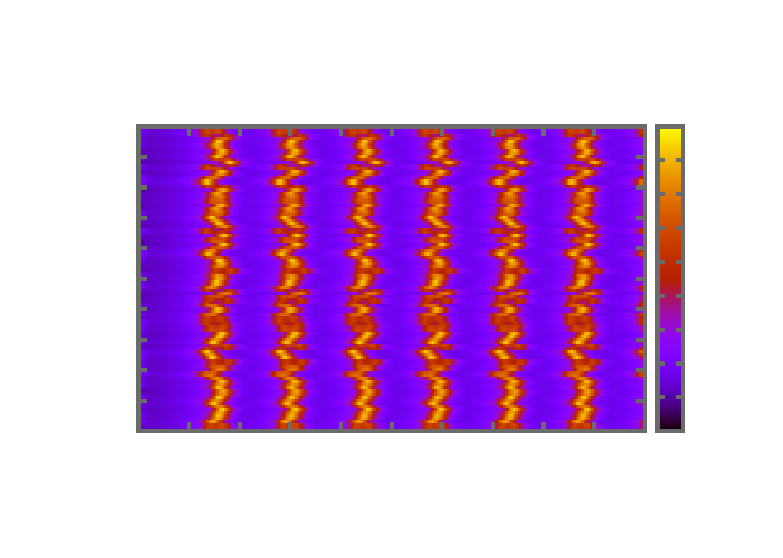
\includegraphics{brussel2}}%
    \gplfronttext
  \end{picture}%
\endgroup
}
            \caption{Development of system in the brusselator model. Note how
            all cells exhibit the same oscillating behaviour, only slightly
            differing in time.}
            \label{fig:br2}
         \end{minipage}
      \end{figure}

      Analysis of the brusselator model shows that a stable oscillating behaviour
      appears when $k_1[A]/k_3[B] \approx 1/3$ and $k_2/k_4 \approx 4/3$. The
      certainty in this claim is however dubious, since the software for
      simulating the model seems to dislike settings of large enough magnitudes.
      Divergence from these settings do however tend to dampen the system,
      driving it towards steady concentrations for $X$ and $Y$ respectively.

      The same dynamics apply for a system holding many cells, as they all in
      the absence of diffusion will abhere to affect each other. Both these
      cases are shown in \cref{fig:br1} and \cref{fig:br2} correspondingly. 


      \begin{figure}[H]
         \vspace*{1cm}
         \hspace*{-2cm}
         \centering
         \begin{minipage}[t]{.6\textwidth}		
            \vspace{0pt}
            \centering
            \resizebox{\columnwidth}{!}{% GNUPLOT: LaTeX picture with Postscript
\begingroup
  \makeatletter
  \providecommand\color[2][]{%
    \GenericError{(gnuplot) \space\space\space\@spaces}{%
      Package color not loaded in conjunction with
      terminal option `colourtext'%
    }{See the gnuplot documentation for explanation.%
    }{Either use 'blacktext' in gnuplot or load the package
      color.sty in LaTeX.}%
    \renewcommand\color[2][]{}%
  }%
  \providecommand\includegraphics[2][]{%
    \GenericError{(gnuplot) \space\space\space\@spaces}{%
      Package graphicx or graphics not loaded%
    }{See the gnuplot documentation for explanation.%
    }{The gnuplot epslatex terminal needs graphicx.sty or graphics.sty.}%
    \renewcommand\includegraphics[2][]{}%
  }%
  \providecommand\rotatebox[2]{#2}%
  \@ifundefined{ifGPcolor}{%
    \newif\ifGPcolor
    \GPcolortrue
  }{}%
  \@ifundefined{ifGPblacktext}{%
    \newif\ifGPblacktext
    \GPblacktexttrue
  }{}%
  % define a \g@addto@macro without @ in the name:
  \let\gplgaddtomacro\g@addto@macro
  % define empty templates for all commands taking text:
  \gdef\gplbacktext{}%
  \gdef\gplfronttext{}%
  \makeatother
  \ifGPblacktext
    % no textcolor at all
    \def\colorrgb#1{}%
    \def\colorgray#1{}%
  \else
    % gray or color?
    \ifGPcolor
      \def\colorrgb#1{\color[rgb]{#1}}%
      \def\colorgray#1{\color[gray]{#1}}%
      \expandafter\def\csname LTw\endcsname{\color{white}}%
      \expandafter\def\csname LTb\endcsname{\color{black}}%
      \expandafter\def\csname LTa\endcsname{\color{black}}%
      \expandafter\def\csname LT0\endcsname{\color[rgb]{1,0,0}}%
      \expandafter\def\csname LT1\endcsname{\color[rgb]{0,1,0}}%
      \expandafter\def\csname LT2\endcsname{\color[rgb]{0,0,1}}%
      \expandafter\def\csname LT3\endcsname{\color[rgb]{1,0,1}}%
      \expandafter\def\csname LT4\endcsname{\color[rgb]{0,1,1}}%
      \expandafter\def\csname LT5\endcsname{\color[rgb]{1,1,0}}%
      \expandafter\def\csname LT6\endcsname{\color[rgb]{0,0,0}}%
      \expandafter\def\csname LT7\endcsname{\color[rgb]{1,0.3,0}}%
      \expandafter\def\csname LT8\endcsname{\color[rgb]{0.5,0.5,0.5}}%
    \else
      % gray
      \def\colorrgb#1{\color{black}}%
      \def\colorgray#1{\color[gray]{#1}}%
      \expandafter\def\csname LTw\endcsname{\color{white}}%
      \expandafter\def\csname LTb\endcsname{\color{black}}%
      \expandafter\def\csname LTa\endcsname{\color{black}}%
      \expandafter\def\csname LT0\endcsname{\color{black}}%
      \expandafter\def\csname LT1\endcsname{\color{black}}%
      \expandafter\def\csname LT2\endcsname{\color{black}}%
      \expandafter\def\csname LT3\endcsname{\color{black}}%
      \expandafter\def\csname LT4\endcsname{\color{black}}%
      \expandafter\def\csname LT5\endcsname{\color{black}}%
      \expandafter\def\csname LT6\endcsname{\color{black}}%
      \expandafter\def\csname LT7\endcsname{\color{black}}%
      \expandafter\def\csname LT8\endcsname{\color{black}}%
    \fi
  \fi
  \setlength{\unitlength}{0.0500bp}%
  \begin{picture}(7200.00,5040.00)%
    \gplgaddtomacro\gplbacktext{%
      \colorrgb{0.42,0.42,0.42}%
      \put(3600,4312){\makebox(0,0){\strut{}}}%
    }%
    \gplgaddtomacro\gplfronttext{%
      \colorrgb{0.42,0.42,0.42}%
      \put(1170,772){\makebox(0,0){\strut{} 0}}%
      \colorrgb{0.42,0.42,0.42}%
      \put(1656,772){\makebox(0,0){\strut{} 2}}%
      \colorrgb{0.42,0.42,0.42}%
      \put(2142,772){\makebox(0,0){\strut{} 4}}%
      \colorrgb{0.42,0.42,0.42}%
      \put(2628,772){\makebox(0,0){\strut{} 6}}%
      \colorrgb{0.42,0.42,0.42}%
      \put(3114,772){\makebox(0,0){\strut{} 8}}%
      \colorrgb{0.42,0.42,0.42}%
      \put(3600,772){\makebox(0,0){\strut{} 10}}%
      \colorrgb{0.42,0.42,0.42}%
      \put(4086,772){\makebox(0,0){\strut{} 12}}%
      \colorrgb{0.42,0.42,0.42}%
      \put(4572,772){\makebox(0,0){\strut{} 14}}%
      \colorrgb{0.42,0.42,0.42}%
      \put(5058,772){\makebox(0,0){\strut{} 16}}%
      \colorrgb{0.42,0.42,0.42}%
      \put(5544,772){\makebox(0,0){\strut{} 18}}%
      \colorrgb{0.42,0.42,0.42}%
      \put(6030,772){\makebox(0,0){\strut{} 20}}%
      \colorrgb{0.42,0.42,0.42}%
      \put(3600,442){\makebox(0,0){\strut{}Time}}%
      \colorrgb{0.42,0.42,0.42}%
      \put(998,1058){\makebox(0,0)[r]{\strut{} 0}}%
      \colorrgb{0.42,0.42,0.42}%
      \put(998,1351){\makebox(0,0)[r]{\strut{} 10}}%
      \colorrgb{0.42,0.42,0.42}%
      \put(998,1643){\makebox(0,0)[r]{\strut{} 20}}%
      \colorrgb{0.42,0.42,0.42}%
      \put(998,1936){\makebox(0,0)[r]{\strut{} 30}}%
      \colorrgb{0.42,0.42,0.42}%
      \put(998,2228){\makebox(0,0)[r]{\strut{} 40}}%
      \colorrgb{0.42,0.42,0.42}%
      \put(998,2520){\makebox(0,0)[r]{\strut{} 50}}%
      \colorrgb{0.42,0.42,0.42}%
      \put(998,2812){\makebox(0,0)[r]{\strut{} 60}}%
      \colorrgb{0.42,0.42,0.42}%
      \put(998,3104){\makebox(0,0)[r]{\strut{} 70}}%
      \colorrgb{0.42,0.42,0.42}%
      \put(998,3397){\makebox(0,0)[r]{\strut{} 80}}%
      \colorrgb{0.42,0.42,0.42}%
      \put(998,3689){\makebox(0,0)[r]{\strut{} 90}}%
      \colorrgb{0.42,0.42,0.42}%
      \put(998,3982){\makebox(0,0)[r]{\strut{} 100}}%
      \colorrgb{0.42,0.42,0.42}%
      \put(404,2520){\rotatebox{-270}{\makebox(0,0){\strut{}Cell}}}%
      \colorrgb{0.42,0.42,0.42}%
      \put(6527,1058){\makebox(0,0)[l]{\strut{} 0}}%
      \colorrgb{0.42,0.42,0.42}%
      \put(6527,1382){\makebox(0,0)[l]{\strut{} 0.2}}%
      \colorrgb{0.42,0.42,0.42}%
      \put(6527,1707){\makebox(0,0)[l]{\strut{} 0.4}}%
      \colorrgb{0.42,0.42,0.42}%
      \put(6527,2032){\makebox(0,0)[l]{\strut{} 0.6}}%
      \colorrgb{0.42,0.42,0.42}%
      \put(6527,2357){\makebox(0,0)[l]{\strut{} 0.8}}%
      \colorrgb{0.42,0.42,0.42}%
      \put(6527,2682){\makebox(0,0)[l]{\strut{} 1}}%
      \colorrgb{0.42,0.42,0.42}%
      \put(6527,3007){\makebox(0,0)[l]{\strut{} 1.2}}%
      \colorrgb{0.42,0.42,0.42}%
      \put(6527,3332){\makebox(0,0)[l]{\strut{} 1.4}}%
      \colorrgb{0.42,0.42,0.42}%
      \put(6527,3657){\makebox(0,0)[l]{\strut{} 1.6}}%
      \colorrgb{0.42,0.42,0.42}%
      \put(6527,3981){\makebox(0,0)[l]{\strut{} 1.8}}%
    }%
    \gplbacktext
    \put(0,0){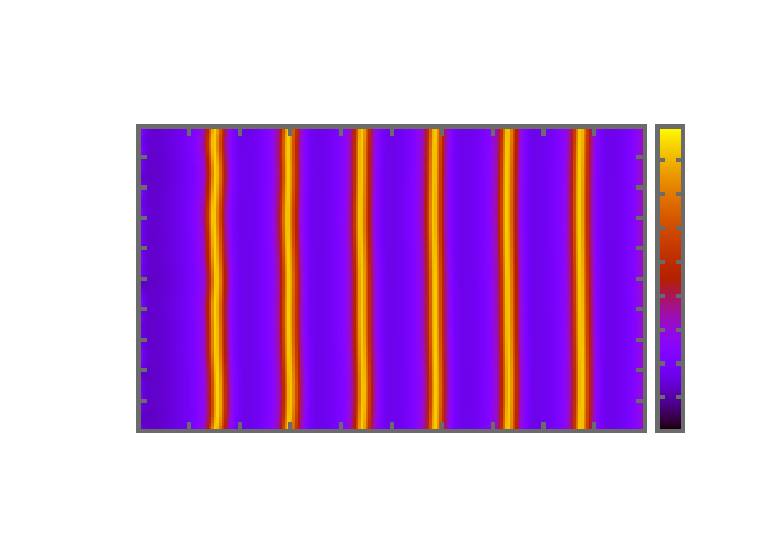
\includegraphics{brussel3}}%
    \gplfronttext
  \end{picture}%
\endgroup
}
            \caption{Brusselator system with the includance of diffusion.
            In comparison to \cref{fig:br2} the smoothness is apparent.}
            \label{fig:br3}
         \end{minipage}~\hspace*{1em}
         \begin{minipage}[t]{.6\textwidth}		
            \vspace{0pt}
            \centering
            \resizebox{\columnwidth}{!}{% GNUPLOT: LaTeX picture with Postscript
\begingroup
  \makeatletter
  \providecommand\color[2][]{%
    \GenericError{(gnuplot) \space\space\space\@spaces}{%
      Package color not loaded in conjunction with
      terminal option `colourtext'%
    }{See the gnuplot documentation for explanation.%
    }{Either use 'blacktext' in gnuplot or load the package
      color.sty in LaTeX.}%
    \renewcommand\color[2][]{}%
  }%
  \providecommand\includegraphics[2][]{%
    \GenericError{(gnuplot) \space\space\space\@spaces}{%
      Package graphicx or graphics not loaded%
    }{See the gnuplot documentation for explanation.%
    }{The gnuplot epslatex terminal needs graphicx.sty or graphics.sty.}%
    \renewcommand\includegraphics[2][]{}%
  }%
  \providecommand\rotatebox[2]{#2}%
  \@ifundefined{ifGPcolor}{%
    \newif\ifGPcolor
    \GPcolortrue
  }{}%
  \@ifundefined{ifGPblacktext}{%
    \newif\ifGPblacktext
    \GPblacktexttrue
  }{}%
  % define a \g@addto@macro without @ in the name:
  \let\gplgaddtomacro\g@addto@macro
  % define empty templates for all commands taking text:
  \gdef\gplbacktext{}%
  \gdef\gplfronttext{}%
  \makeatother
  \ifGPblacktext
    % no textcolor at all
    \def\colorrgb#1{}%
    \def\colorgray#1{}%
  \else
    % gray or color?
    \ifGPcolor
      \def\colorrgb#1{\color[rgb]{#1}}%
      \def\colorgray#1{\color[gray]{#1}}%
      \expandafter\def\csname LTw\endcsname{\color{white}}%
      \expandafter\def\csname LTb\endcsname{\color{black}}%
      \expandafter\def\csname LTa\endcsname{\color{black}}%
      \expandafter\def\csname LT0\endcsname{\color[rgb]{1,0,0}}%
      \expandafter\def\csname LT1\endcsname{\color[rgb]{0,1,0}}%
      \expandafter\def\csname LT2\endcsname{\color[rgb]{0,0,1}}%
      \expandafter\def\csname LT3\endcsname{\color[rgb]{1,0,1}}%
      \expandafter\def\csname LT4\endcsname{\color[rgb]{0,1,1}}%
      \expandafter\def\csname LT5\endcsname{\color[rgb]{1,1,0}}%
      \expandafter\def\csname LT6\endcsname{\color[rgb]{0,0,0}}%
      \expandafter\def\csname LT7\endcsname{\color[rgb]{1,0.3,0}}%
      \expandafter\def\csname LT8\endcsname{\color[rgb]{0.5,0.5,0.5}}%
    \else
      % gray
      \def\colorrgb#1{\color{black}}%
      \def\colorgray#1{\color[gray]{#1}}%
      \expandafter\def\csname LTw\endcsname{\color{white}}%
      \expandafter\def\csname LTb\endcsname{\color{black}}%
      \expandafter\def\csname LTa\endcsname{\color{black}}%
      \expandafter\def\csname LT0\endcsname{\color{black}}%
      \expandafter\def\csname LT1\endcsname{\color{black}}%
      \expandafter\def\csname LT2\endcsname{\color{black}}%
      \expandafter\def\csname LT3\endcsname{\color{black}}%
      \expandafter\def\csname LT4\endcsname{\color{black}}%
      \expandafter\def\csname LT5\endcsname{\color{black}}%
      \expandafter\def\csname LT6\endcsname{\color{black}}%
      \expandafter\def\csname LT7\endcsname{\color{black}}%
      \expandafter\def\csname LT8\endcsname{\color{black}}%
    \fi
  \fi
  \setlength{\unitlength}{0.0500bp}%
  \begin{picture}(7200.00,5040.00)%
    \gplgaddtomacro\gplbacktext{%
      \colorrgb{0.42,0.42,0.42}%
      \put(3600,4312){\makebox(0,0){\strut{}}}%
    }%
    \gplgaddtomacro\gplfronttext{%
      \colorrgb{0.42,0.42,0.42}%
      \put(1170,772){\makebox(0,0){\strut{} 0}}%
      \colorrgb{0.42,0.42,0.42}%
      \put(1777,772){\makebox(0,0){\strut{} 100}}%
      \colorrgb{0.42,0.42,0.42}%
      \put(2385,772){\makebox(0,0){\strut{} 200}}%
      \colorrgb{0.42,0.42,0.42}%
      \put(2993,772){\makebox(0,0){\strut{} 300}}%
      \colorrgb{0.42,0.42,0.42}%
      \put(3600,772){\makebox(0,0){\strut{} 400}}%
      \colorrgb{0.42,0.42,0.42}%
      \put(4207,772){\makebox(0,0){\strut{} 500}}%
      \colorrgb{0.42,0.42,0.42}%
      \put(4815,772){\makebox(0,0){\strut{} 600}}%
      \colorrgb{0.42,0.42,0.42}%
      \put(5423,772){\makebox(0,0){\strut{} 700}}%
      \colorrgb{0.42,0.42,0.42}%
      \put(6030,772){\makebox(0,0){\strut{} 800}}%
      \colorrgb{0.42,0.42,0.42}%
      \put(3600,442){\makebox(0,0){\strut{}Time}}%
      \colorrgb{0.42,0.42,0.42}%
      \put(998,1058){\makebox(0,0)[r]{\strut{} 0}}%
      \colorrgb{0.42,0.42,0.42}%
      \put(998,1351){\makebox(0,0)[r]{\strut{} 5}}%
      \colorrgb{0.42,0.42,0.42}%
      \put(998,1643){\makebox(0,0)[r]{\strut{} 10}}%
      \colorrgb{0.42,0.42,0.42}%
      \put(998,1936){\makebox(0,0)[r]{\strut{} 15}}%
      \colorrgb{0.42,0.42,0.42}%
      \put(998,2228){\makebox(0,0)[r]{\strut{} 20}}%
      \colorrgb{0.42,0.42,0.42}%
      \put(998,2520){\makebox(0,0)[r]{\strut{} 25}}%
      \colorrgb{0.42,0.42,0.42}%
      \put(998,2812){\makebox(0,0)[r]{\strut{} 30}}%
      \colorrgb{0.42,0.42,0.42}%
      \put(998,3104){\makebox(0,0)[r]{\strut{} 35}}%
      \colorrgb{0.42,0.42,0.42}%
      \put(998,3397){\makebox(0,0)[r]{\strut{} 40}}%
      \colorrgb{0.42,0.42,0.42}%
      \put(998,3689){\makebox(0,0)[r]{\strut{} 45}}%
      \colorrgb{0.42,0.42,0.42}%
      \put(998,3982){\makebox(0,0)[r]{\strut{} 50}}%
      \colorrgb{0.42,0.42,0.42}%
      \put(536,2520){\rotatebox{-270}{\makebox(0,0){\strut{}Cell}}}%
      \colorrgb{0.42,0.42,0.42}%
      \put(6527,1058){\makebox(0,0)[l]{\strut{} 0}}%
      \colorrgb{0.42,0.42,0.42}%
      \put(6527,1545){\makebox(0,0)[l]{\strut{} 0.5}}%
      \colorrgb{0.42,0.42,0.42}%
      \put(6527,2032){\makebox(0,0)[l]{\strut{} 1}}%
      \colorrgb{0.42,0.42,0.42}%
      \put(6527,2520){\makebox(0,0)[l]{\strut{} 1.5}}%
      \colorrgb{0.42,0.42,0.42}%
      \put(6527,3007){\makebox(0,0)[l]{\strut{} 2}}%
      \colorrgb{0.42,0.42,0.42}%
      \put(6527,3494){\makebox(0,0)[l]{\strut{} 2.5}}%
      \colorrgb{0.42,0.42,0.42}%
      \put(6527,3982){\makebox(0,0)[l]{\strut{} 3}}%
    }%
    \gplbacktext
    \put(0,0){\includegraphics{brussel4}}%
    \gplfronttext
  \end{picture}%
\endgroup
}
            \caption{With only the second diffusion parameter set, the system
            oscillates heavily before all cells reach steady states.}
            \label{fig:br4}
         \end{minipage}
      \end{figure}

      When diffusion instead is introduced, the oscillations smoothen out as in
      \cref{fig:br3}, showing that the system is more heavily driven by the
      dynamics caused by the reaction rates for smaller diffusion rates. 

      A steady state is once again realised when diffusion only is allowed to
      happen for the substrate $Y$, after some initial oscillating. This ought
      to be due to the equation system introduced in the brusselator model
      assuming a self-maintaing equilibrium state at a certain
      concentration for $X$ and $Y$, such that all derivatives with respect to
      time are effectively zero.  

      When the diffusion rates for both $X$ and $Y$ instead are equal or biased
      towards the $D_X \gg D_Y$, and of
      magnitude where the system does not break, the model tends to assume and
      maintain an ongoing oscillating behaviour. In particular, when
      examining the concentrations over all cells at a single time step this
      sinusoidal tendency is apparent. In other words, it emphasises how the
      diffusive tendencies push the concentration from one end of the spectrum
      to the other, in a periodical manner.

      In conclusion, it is clear that chemical reactions can extensively be
      explained by different models, where the amount of details taken
      into account heavily will determine the final behaviour, and in effect
      render results more or less accurate to this correspondingly. We can
      however in our cases adjust our model accordingly to achieve the intended
      behaviour. As a consequence we can furthermore investigate even wider
      implications of our model, as in the brusselator case where
      the complex nature of pattern forming appears.

      The dynamics, and in particular the equilibriums and \textit{states}, 
      of our chemical reactions can indeed to a
      high extent be explained and modeled by statistical probabilities and
      energetic compositions. When a large amount of different substances are of
      essence in the analysis, our numerical methods are certainly prefereable,
      as the analytical case would contain numerous coupled differential
      equations.

\begin{thebibliography}{99}
   \bibitem{lecnotes}
     Bozorg, Behruz,
     \emph{Computer Assignment 2: Chemical reaction networks and diffusion},
     Lund University,
     2015.
   \bibitem{nelson}
     Nelson, Philip,
     \emph{Biological Physics: Energy, Information, Life},
     W.H. Freeman and Company,
     New York,
     2008.
\end{thebibliography}
\end{document}

